\documentclass{beamer}
\usetheme{metropolis}           % Use metropolis theme
\usepackage{appendixnumberbeamer}
\usepackage{epigraph}
\usepackage{color}
\usepackage{amsopn}
\usepackage{tabto}
\usepackage{pbox}           % table line break
\usepackage{algorithm}      % algorithm
\usepackage[noend]{algpseudocode} % algorithm
\usepackage{bm}             % bold in math
\usepackage{mathtools}      % dcases*

\usepackage{booktabs}       % professional-quality tables
\usepackage{amsfonts}       % blackboard math symbols
\usepackage{amsmath}
\usepackage{amssymb}
\usepackage{nicefrac}       % compact symbols for 1/2, etc.
\usepackage{microtype}      % microtypography
\usepackage{graphicx}
\usepackage{subcaption}
\usepackage{multirow}
\usepackage{makecell}

%%% Bibliography
\usepackage[backend=bibtex, style=authoryear]{biblatex}
\AtBeginBibliography{\tiny}
\bibliography{../bibliography.bib}

\setcounter{tocdepth}{1}      % hide subsections in Table of Contents
\renewcommand{\thealgorithm}{} % disable numbering of algorithms

\setbeamercolor{background canvas}{bg=white}
\setbeamercolor{title}{fg=black}
\setbeamercolor{subtitle}{fg=black}
\setbeamercolor{date}{fg=black}
\setbeamercolor{author}{fg=black}
\setbeamercolor{institute}{fg=black}

\newcommand{\todo}{\alert{TODO}}
\newcommand{\itemBullet}{\scriptsize$\blacksquare$}
\setbeamertemplate{itemize item}{\itemBullet}
\setbeamertemplate{itemize subitem}{\itemBullet}
\setbeamertemplate{itemize subsubitem}{\itemBullet}
\newcommand{\E}{\mathop{\mathbb{E}}}
\DeclareMathOperator*{\argmax}{arg\,max}
\newcommand{\epiParSpace}{\vskip 1.5ex}
\newcommand{\p}{\mathbf{p}}
\newcommand{\colorcite}{\color{gray!35}}
\newcolumntype{?}[1]{!{\vrule width #1}}
\newcommand{\hbline}{\Xhline{2.5\arrayrulewidth}}
\newcommand\nocell[1]{\multicolumn{#1}{c?{1.5pt}}{}}
\setcellgapes{5pt}

\newcommand{\atariCitation}{\colorcite[\cite{Mnih2015human}]}
\newcommand{\cepheusCitation}{\colorcite[\cite{Bowling2015heads}]}
\newcommand{\alphaGoCitation}{\colorcite[\cite{Silver2016mastering}]}
\newcommand{\searchTreeCitation}{\colorcite[\cite{Allis1994searching}]}
\newcommand{\nnModesCitation}{\colorcite[\cite{Dieterle2003multianalyte}]}
\newcommand{\deepstackAiCitation}{\colorcite\url{https://www.deepstack.ai}}
\newcommand{\deepStackCitation}{\colorcite[\cite{Moravcik2017deepstack}]}

\title{\Huge AI Supremacy in Games}
\subtitle{\small Deep Blue, Watson, Cepheus, AlphaGo, DeepStack and TensorCFR}
\date{13\textsuperscript{th} June 2018}
\author{Karel Ha}
\institute{Artificial Intelligence Center\\
  Czech Technical University in Prague}

\begin{document}
  {
    \usebackgroundtemplate{
      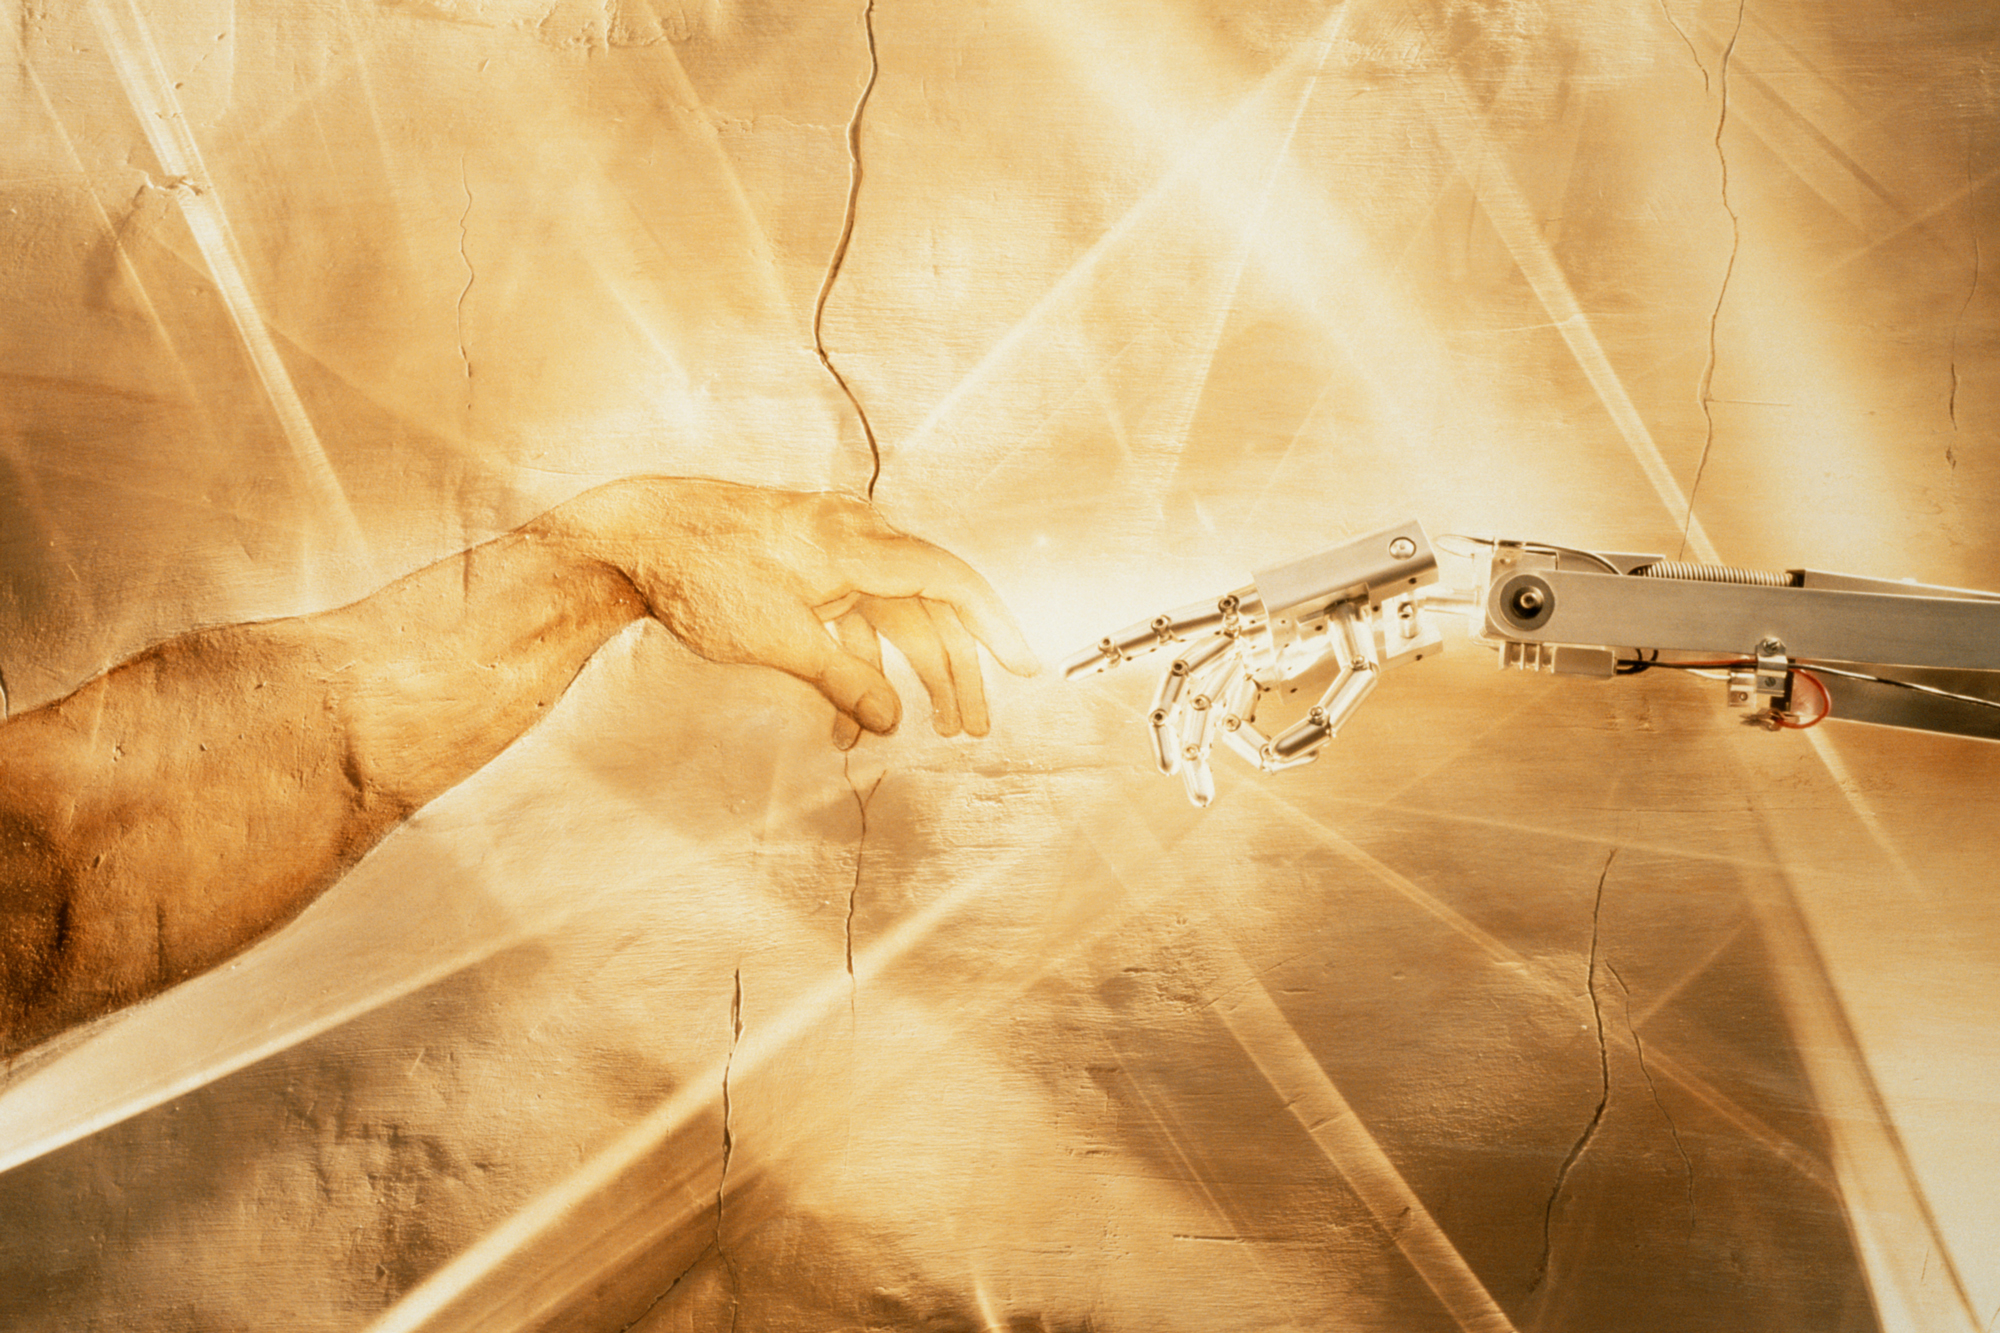
\includegraphics[height=\paperheight]{../img/hands-touch-of-god.jpg}
    }
    \maketitle
  }

  \begin{frame}{The Outline}
    \tableofcontents
  \end{frame}

%%%%%%%%%%%%%%%%%%%%%%%%%%%%%%%%%%%%%%%%%%%%%%%%%%%%%%%%%%%%%%%%%%%%%%%%%%%%%%%%

  \section{General AI: One Summer Dream}

%%%%%%%%%%%%%%%%%%%%%%%%%%%%%%%%%%%%%%%%%%%%%%%%%%%%%%%%%%%%%%%%%%%%%%%%%%%%%%%%

  \section{AI in Games}
  \begin{frame}[standout]
    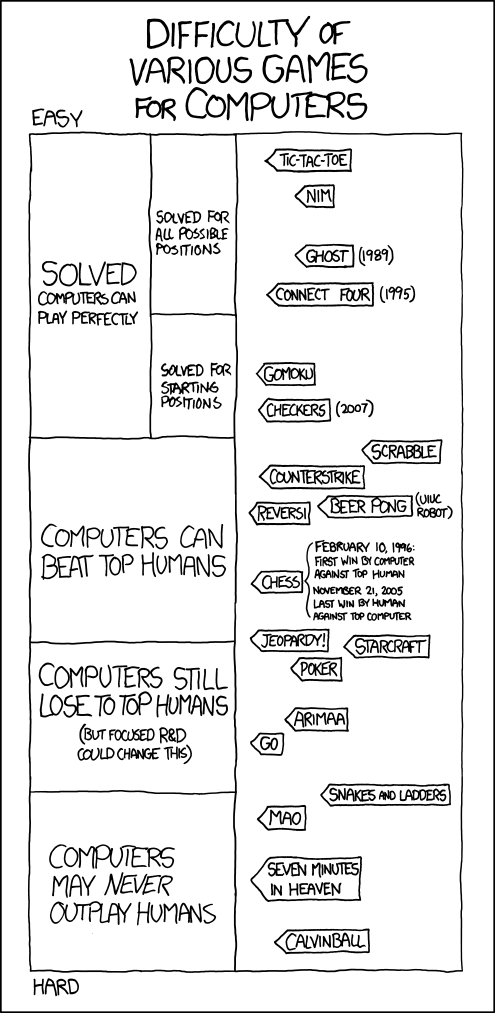
\includegraphics[height=\paperheight]{../img/game_AIs.png}
    \nocite{xkcdGameAIs}
  \end{frame}

%%%%%%%%%%%%%%%%%%%%%%%%%%%%%%%%%%%%%%%%%%%%%%%%%%%%%%%%%%%%%%%%%%%%%%%%%%%%%%%%

  \section{Chess: Deep Blue}

%%%%%%%%%%%%%%%%%%%%%%%%%%%%%%%%%%%%%%%%%%%%%%%%%%%%%%%%%%%%%%%%%%%%%%%%%%%%%%%%

  \section{Jeopardy!: Watson}

%%%%%%%%%%%%%%%%%%%%%%%%%%%%%%%%%%%%%%%%%%%%%%%%%%%%%%%%%%%%%%%%%%%%%%%%%%%%%%%%

  \section{Atari Games:\\
    Deep Reinforcement Learning}
  {
    \setbeamertemplate{frame footer}{\atariCitation}
    \begin{frame}{Atari Player by Google DeepMind}
      \begin{center}
        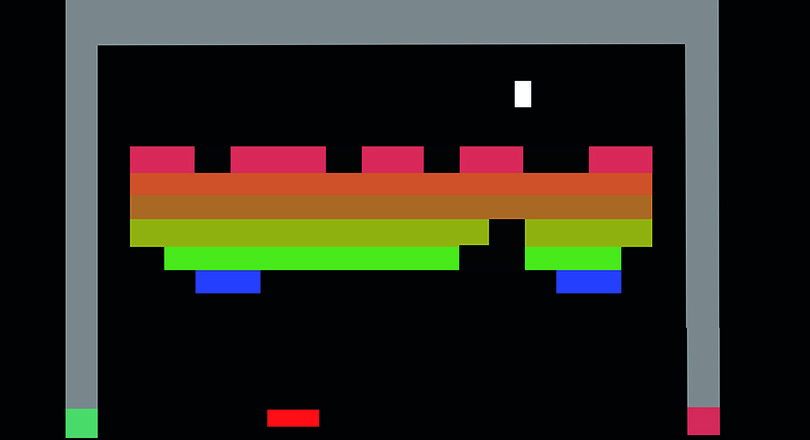
\includegraphics[width=\textwidth, height=\textheight, keepaspectratio]{../img/atari_breakout.jpg}

        \url{https://youtu.be/0X-NdPtFKq0?t=21m13s}
      \end{center}
    \end{frame}
  }

  {
    \setbeamertemplate{frame footer}{\url{https://youtu.be/0X-NdPtFKq0?t=16m57s}}
    \begin{frame}{Reinforcement Learning}
      \begin{center}
        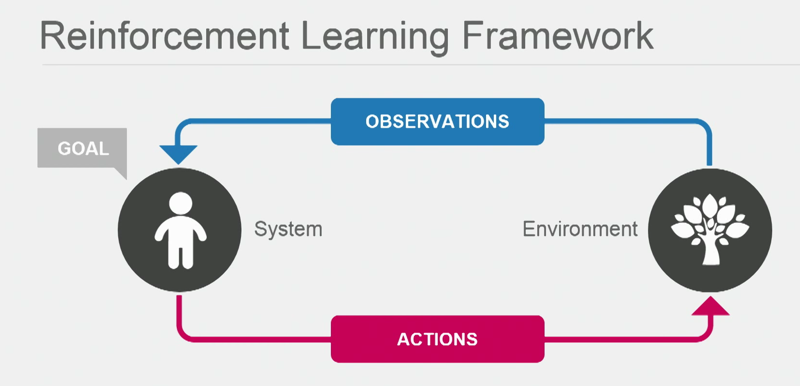
\includegraphics[width=\textwidth]{../img/RL_framework.png}
      \end{center}
      \pause
      games of \textbf{self-play}
    \end{frame}
  }

%%%%%%%%%%%%%%%%%%%%%%%%%%%%%%%%%%%%%%%%%%%%%%%%%%%%%%%%%%%%%%%%%%%%%%%%%%%%%%%%

  \section{Go:\\
    AlphaGo, AlphaGo Zero, AlphaZero}

  \begin{frame}[standout]
    \begin{center}
      Crash Course:\\
      Tree Search
    \end{center}
  \end{frame}

  {
    \setbeamertemplate{frame footer}{\alphaGoCitation}
    \begin{frame}{Tree Search}
      Optimal value~$v^*(s)$ determines the~outcome of~the game:
      \pause
      \begin{itemize}[<+- | alert@+>]
          \tiny
        \item from every board position or state $s$
        \item under perfect play by~all players.
      \end{itemize}
      \pause

      It is computed by~\textbf{recursively traversing a~search tree} containing approximately $b^d$ possible sequences of moves, where
      \pause
      \begin{itemize}[<+- | alert@+>]
          \tiny
        \item $b$ is the game’s breadth (number of legal moves per position)
        \item $d$ is its depth (game length)
      \end{itemize}
    \end{frame}
  }

  {
    \setbeamertemplate{frame footer}{\searchTreeCitation}
    \begin{frame}{Game tree of~Go}
      Sizes of~trees for~various games:
      \begin{itemize}
        \item chess: $b \approx 35, d \approx 80$
        \item Go: $b \approx 250, d \approx 150$
          \pause
          $\Rightarrow$ more positions than atoms in the universe!
      \end{itemize}
      \pause

      \epigraph{
        That makes Go a \textbf{googol} times more complex than chess.
      }{\tiny\url{https://deepmind.com/alpha-go.html}}
      \pause

      \vskip -1em
      How to handle the size~of the game tree?
      \pause
      \begin{itemize}[<+- | alert@+>]
        \item for the breadth: a~neural network to~select moves
        \item for the depth: a~neural network to~evaluate current position
        \item for the tree traverse: Monte Carlo tree search (MCTS)
      \end{itemize}
    \end{frame}
  }

  \begin{frame}{Monte Carlo tree search}
    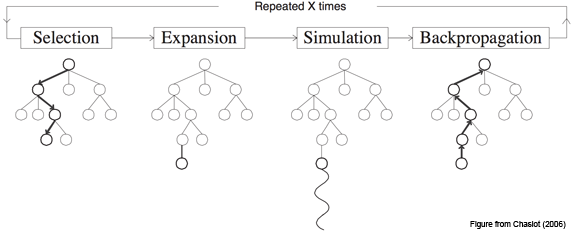
\includegraphics[width=\textwidth]{../img/MCTS.png}
  \end{frame}

  \begin{frame}[standout]
    \begin{center}
      Crash Course:\\
      Neural Networks
    \end{center}
  \end{frame}

  {
    \setbeamertemplate{frame footer}{\url{http://pages.cs.wisc.edu/~bolo/shipyard/neural/local.html}}
    \begin{frame}{Neural Network: Inspiration}
      \vskip -2em
      \begin{center}
        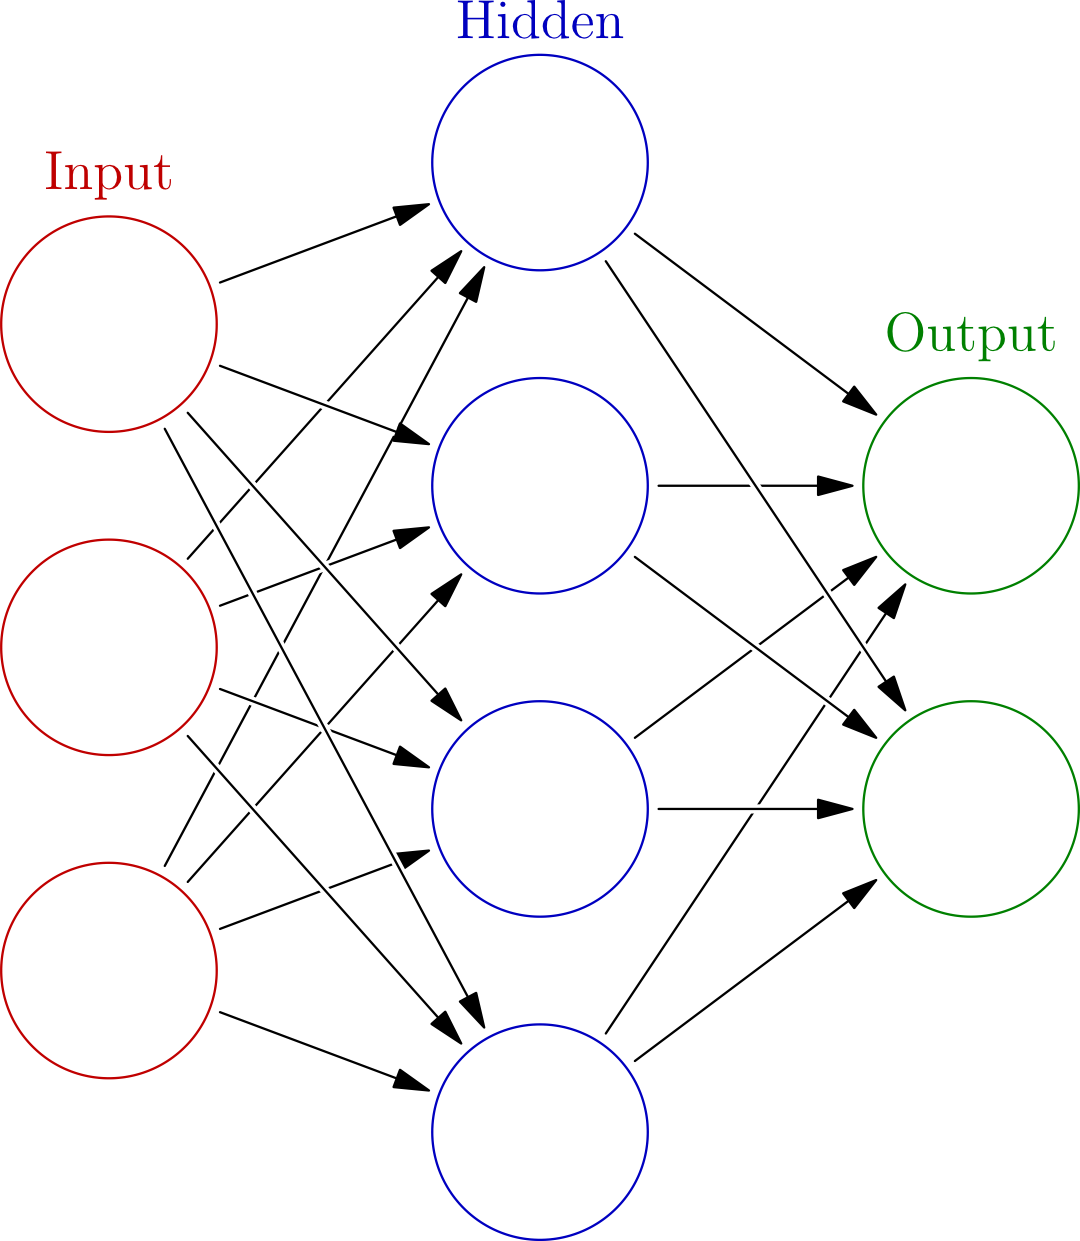
\includegraphics[height=.5\textheight]{../img/colored_neural_network.png}
      \end{center}

      \pause
      \begin{itemize}[<+- | alert@+>]
        \item inspired by~the neuronal structure of~the mammalian cerebral cortex
        \item but on~much smaller scales
        \item suitable to model systems with a~high tolerance to~error 
          \begin{itemize}
            \item e.g.~audio or~image recognition
          \end{itemize}
      \end{itemize}
    \end{frame}
  }

  {
    \setbeamertemplate{frame footer}{\nnModesCitation}
    \begin{frame}{Neural Network: Modes}
      \begin{center}
        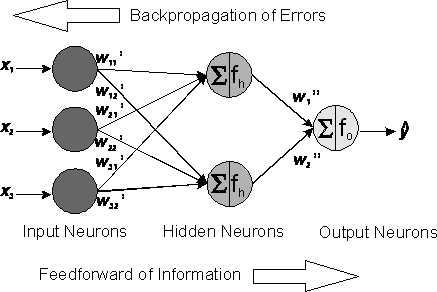
\includegraphics[height=.6\textheight]{../img/neural_network_forward_and_backprop.png}
      \end{center}

      \pause
      Two modes
      \pause
      \begin{itemize}[<+- | alert@+>]
        \item \textbf{feedforward} for making predictions
        \item \textbf{backpropagation} for learning
      \end{itemize}
    \end{frame}
  }

  {
    \setbeamertemplate{frame footer}{\url{http://pages.cs.wisc.edu/~bolo/shipyard/neural/local.html}}

    \begin{frame}{(Deep) Convolutional Neural Network}
      \pause
      \begin{center}
        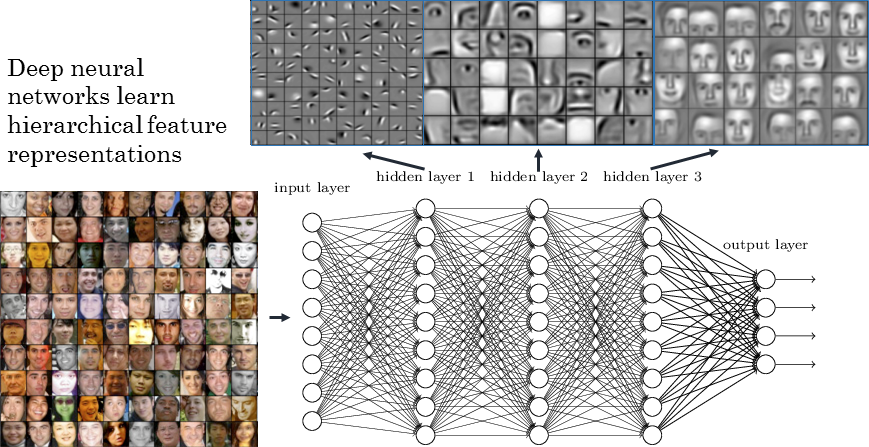
\includegraphics[width=\textwidth]{../img/ConvNet_hierarchy.png}
      \end{center}
    \end{frame}
  }

  \begin{frame}[standout]
    \begin{center}
      AlphaGo
    \end{center}
  \end{frame}

  {
    \setbeamertemplate{frame footer}{\alphaGoCitation}
    \begin{frame}{Policy and Value Networks}
      \begin{center}
        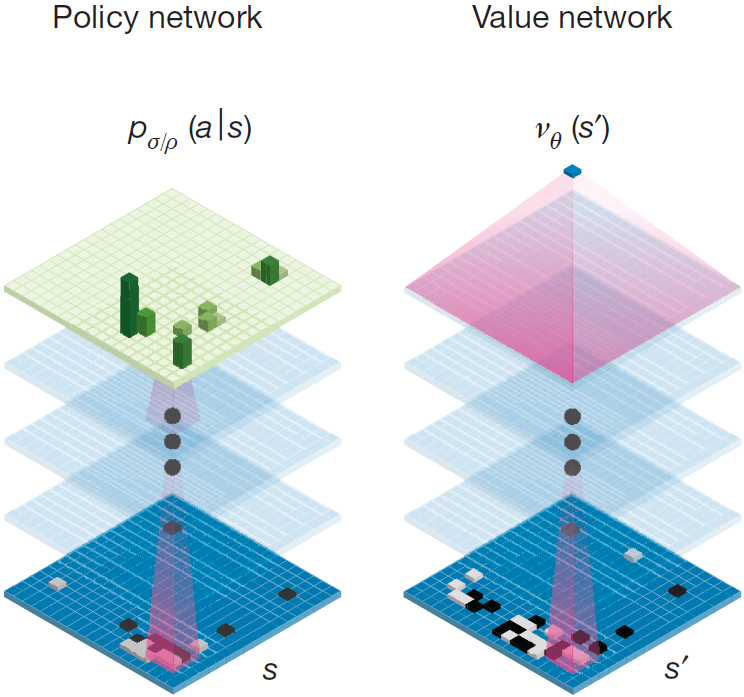
\includegraphics[height=.85\textheight]{../img/policy_and_value_network.png}
      \end{center}
    \end{frame}

    \begin{frame}{Training the (Deep Convolutional) Neural Networks}
      \begin{center}
        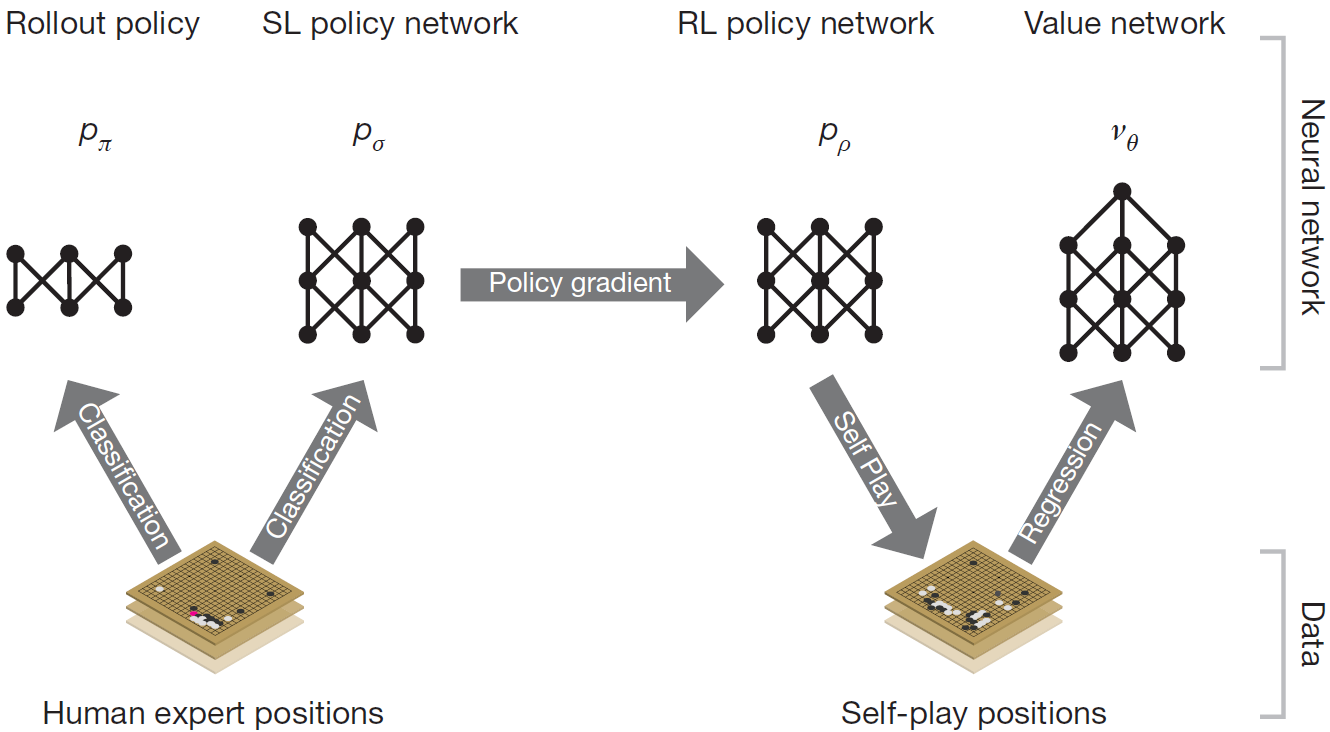
\includegraphics[width=\textwidth]{../img/neural_nets_pipeline.png}
      \end{center}
    \end{frame}

    \begin{frame}{SL Policy Networks}
      \begin{center}
        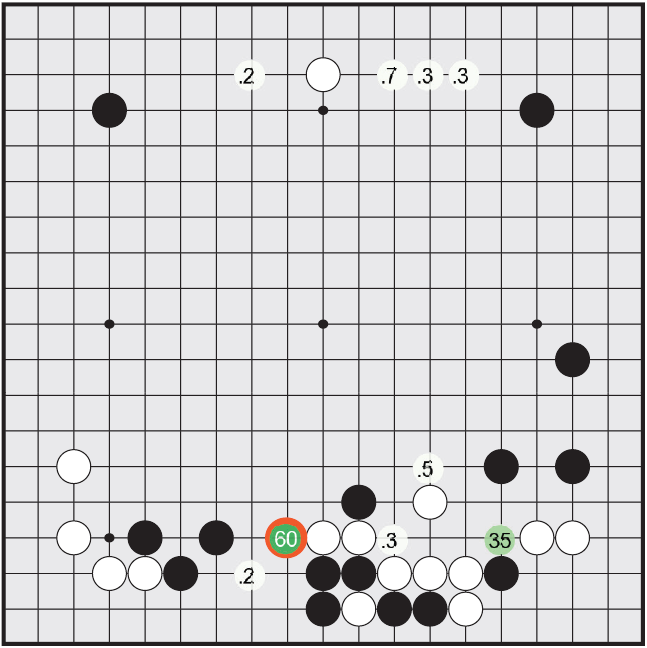
\includegraphics[height=.8\textheight]{../img/eval_SL_policy_network.png}

        \tiny
        move probabilities taken directly from the SL policy network $p_\sigma$ (reported as a~percentage if above $0.1\%$).
      \end{center}
    \end{frame}

    \begin{frame}{Training the (Deep Convolutional) Neural Networks}
      \begin{center}
        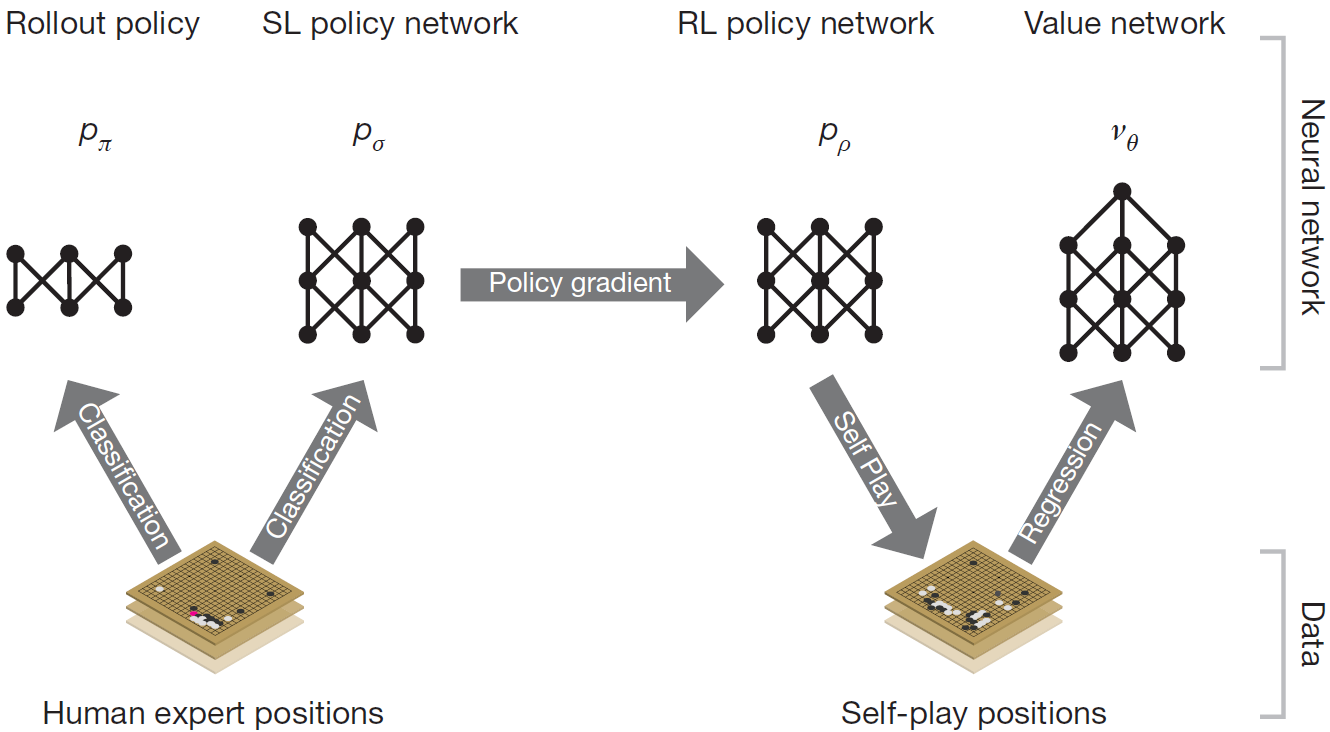
\includegraphics[width=\textwidth]{../img/neural_nets_pipeline.png}
      \end{center}
    \end{frame}

    \begin{frame}{Rollout Policy}
      \begin{itemize}[<+- | alert@+>]
        \item Rollout policy~$p_\pi(a|s)$ is \textbf{faster} but \textbf{less accurate} than SL policy network.
        \item It takes $2 \mu$s to~select an~action, compared to $3$~ms in~case of~SL policy network.
      \end{itemize}
    \end{frame}

    \begin{frame}{Training the (Deep Convolutional) Neural Networks}
      \begin{center}
        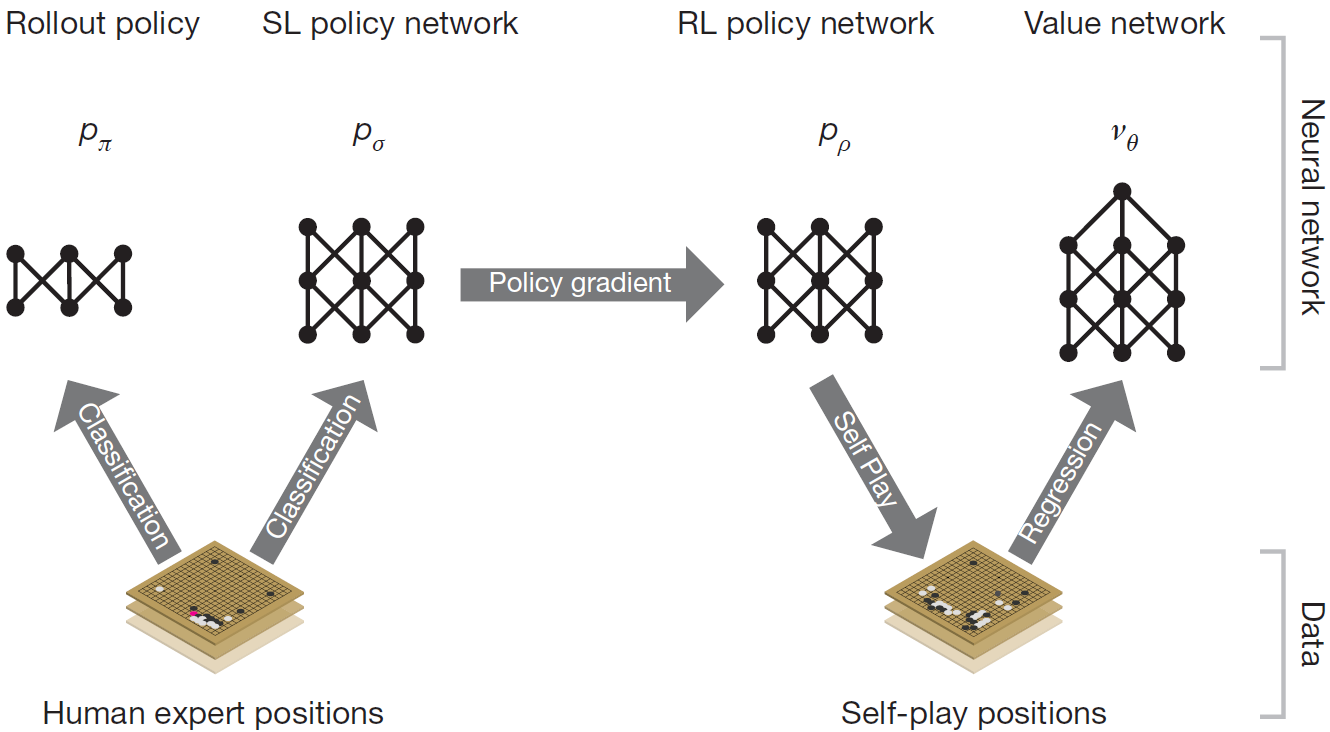
\includegraphics[width=\textwidth]{../img/neural_nets_pipeline.png}
      \end{center}
    \end{frame}

    \begin{frame}{RL Policy Networks}
      \begin{itemize}[<+- | alert@+>]
        \item identical in~structure to the SL policy network
        \item games of \textbf{self-play}
          \begin{itemize}[<+- | alert@+>]
            \item between the current RL policy network and a~randomly selected previous iteration
            \item goal: to~win in~the games of~self-play
          \end{itemize}
      \end{itemize}
      \pause
    \end{frame}

    \begin{frame}{Training the (Deep Convolutional) Neural Networks}
      \begin{center}
        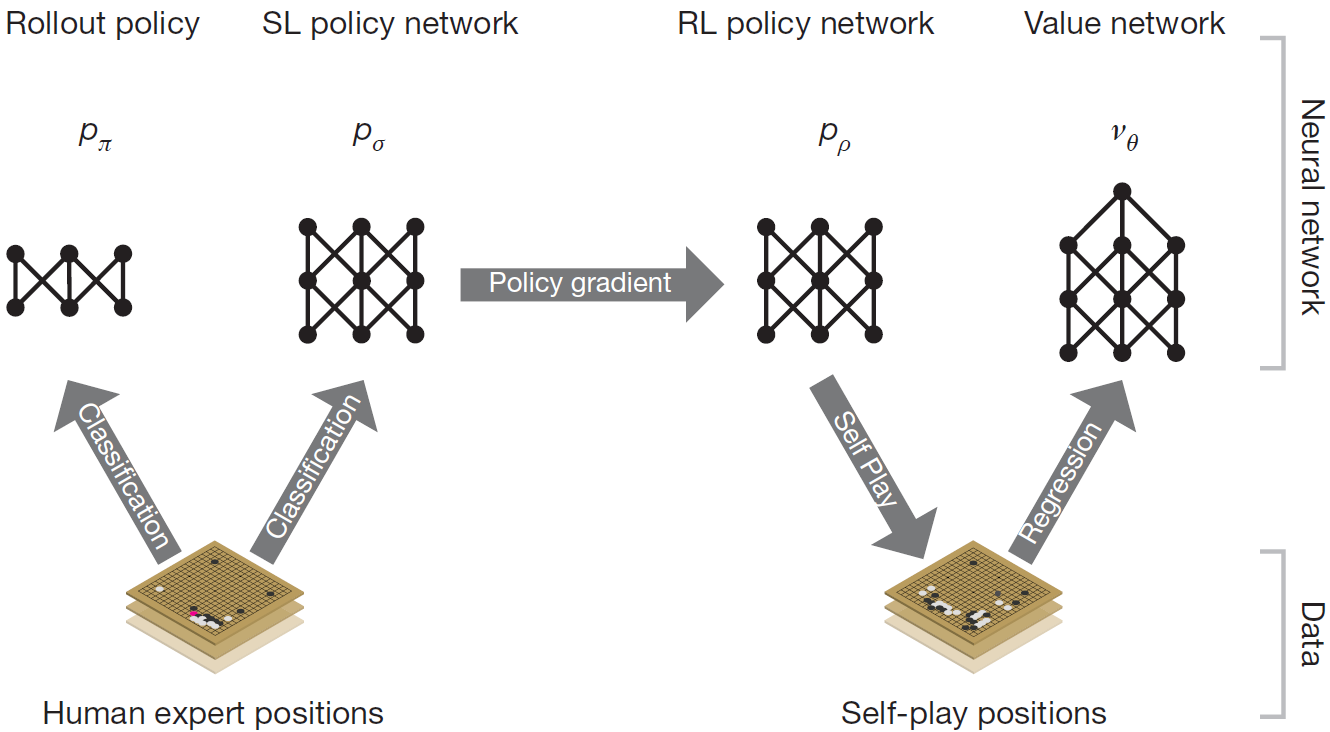
\includegraphics[width=\textwidth]{../img/neural_nets_pipeline.png}
      \end{center}
    \end{frame}

    \begin{frame}{Value Network}
      \begin{itemize}[<+- | alert@+>]
        \item similar architecture to the policy network, but outputs a~single prediction instead of~a~probability distribution
        \item Beware: successive positions are strongly correlated!
        \item Value network memorized the game outcomes, rather than generalizing to new positions.
        \item Solution: generate 30 million (new) positions, each sampled from a~\textbf{separate} game
        \item almost the accuracy of~Monte Carlo rollouts (using $p_\rho$), but $15000$ times less computation!
      \end{itemize}
      \pause
    \end{frame}

    \begin{frame}{Value Network: Selection of~Moves}
      \begin{center}
        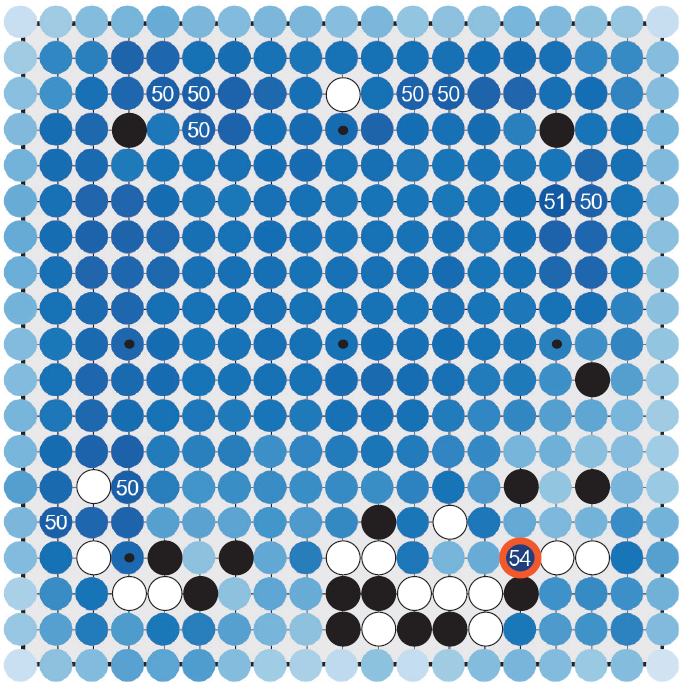
\includegraphics[height=.8\textheight]{../img/move_selection_by_value_network.png}

        \tiny
        evaluation of~all successors $s'$ of~the root position~$s$, using~$v_\theta(s′)$
      \end{center}
    \end{frame}

    \begin{frame}{Training the (Deep Convolutional) Neural Networks}
      \begin{center}
        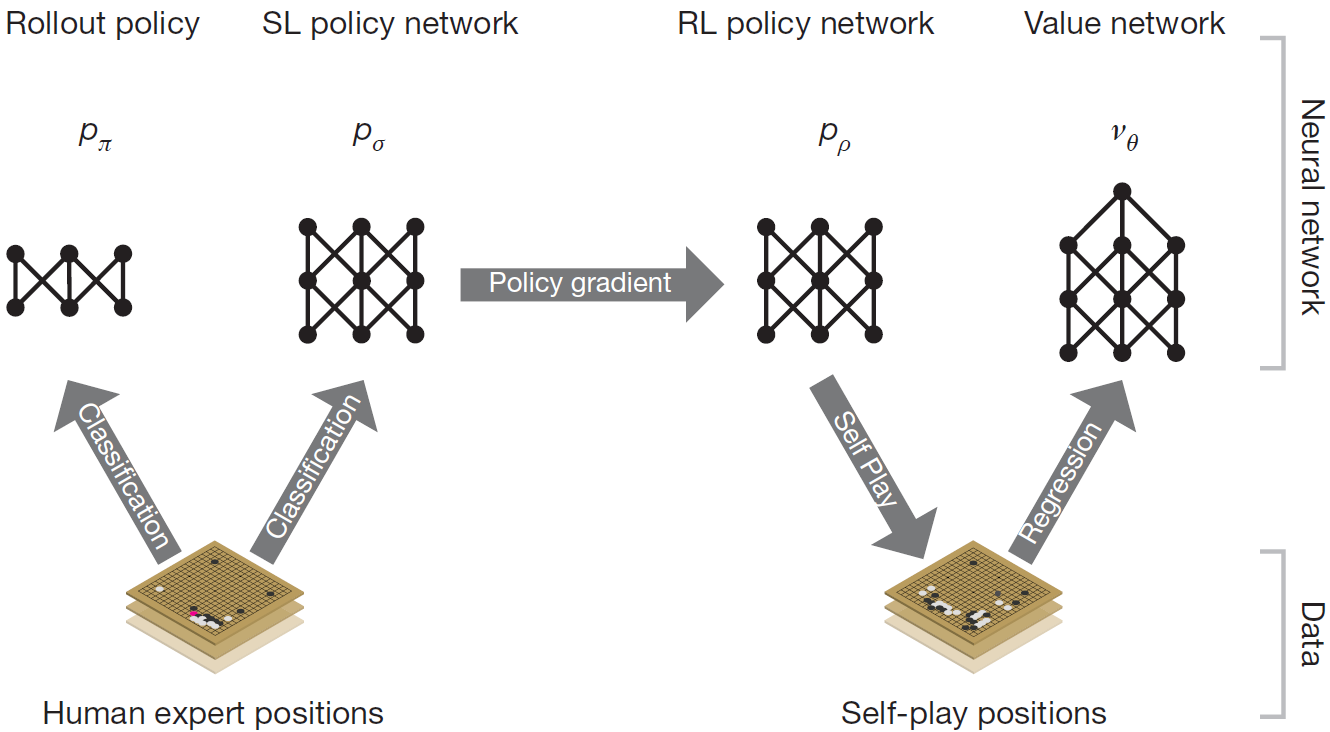
\includegraphics[width=\textwidth]{../img/neural_nets_pipeline.png}
      \end{center}
    \end{frame}

    \begin{frame}{ELO Ratings for~Various Combinations of~Networks}
      \begin{center}
        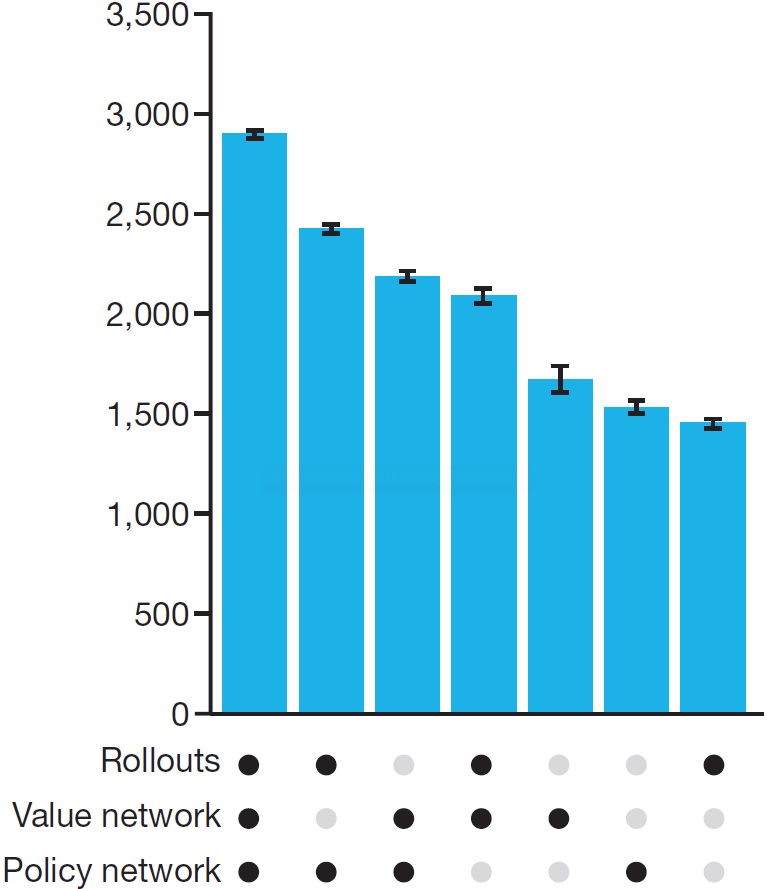
\includegraphics[height=.85\textheight]{../img/ELO_ratings_various_combinations_of_ANNs.png}
      \end{center}
    \end{frame}

    \begin{frame}{Monte Carlo Tree Search (MCTS) Algorithm}
      The tree is traversed by simulation from the root state (i.e. descending the tree).
      \pause

      The next action is selected with a~\textbf{lookahead} search:
      \pause
      \begin{enumerate}[<+- | alert@+>]
        \item selection phase
        \item expansion phase
        \item evaluation phase
        \item backup phase (at~end of~simulation)
          \pause
      \end{enumerate}
    \end{frame}

    \begin{frame}{MCTS Algorithm: Selection}
      \begin{center}
        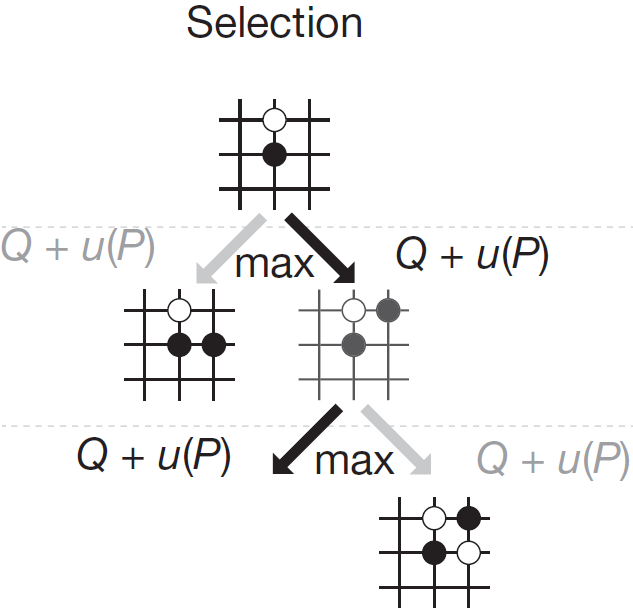
\includegraphics[height=.6\textheight]{../img/MCTS_selection.png}
      \end{center}
    \end{frame}

    \begin{frame}{MCTS Algorithm: Expansion}
      \begin{center}
        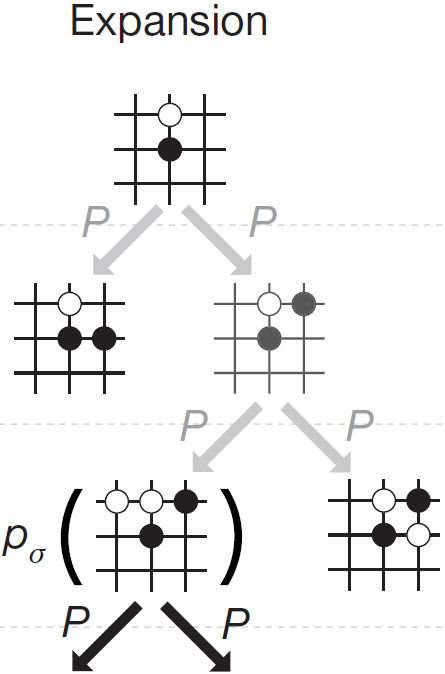
\includegraphics[height=.6\textheight]{../img/MCTS_expansion.png}
      \end{center}
      \pause

      \begin{itemize}[<+- | alert@+>]
        \item A~leaf position may be expanded by the SL policy network~$p_\sigma$.
        \item Once it's expanded, it remains so until the end.
      \end{itemize}
    \end{frame}

    \begin{frame}{MCTS: Evaluation}
      \begin{center}
        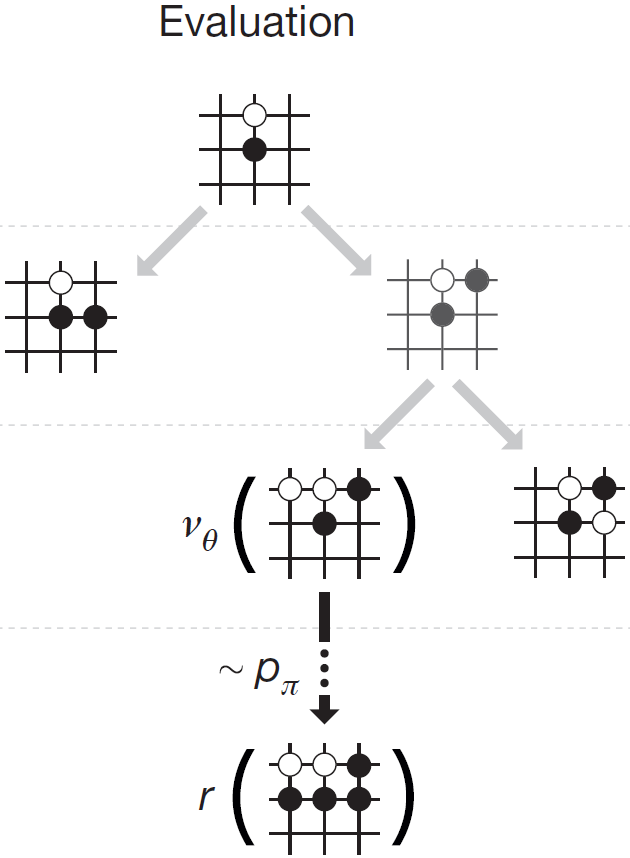
\includegraphics[height=.55\textheight]{../img/MCTS_evaluation.png}
      \end{center}
      \pause

      Both of the following 2 evalutions:
      \pause
      \begin{itemize}[<+- | alert@+>]
        \item evaluation from the value network $v_\theta (s)$
        \item evaluation by the outcome of~the fast rollout $p_\pi$
      \end{itemize}
      \pause
    \end{frame}

    \begin{frame}{MCTS: Backup}
      \begin{center}
        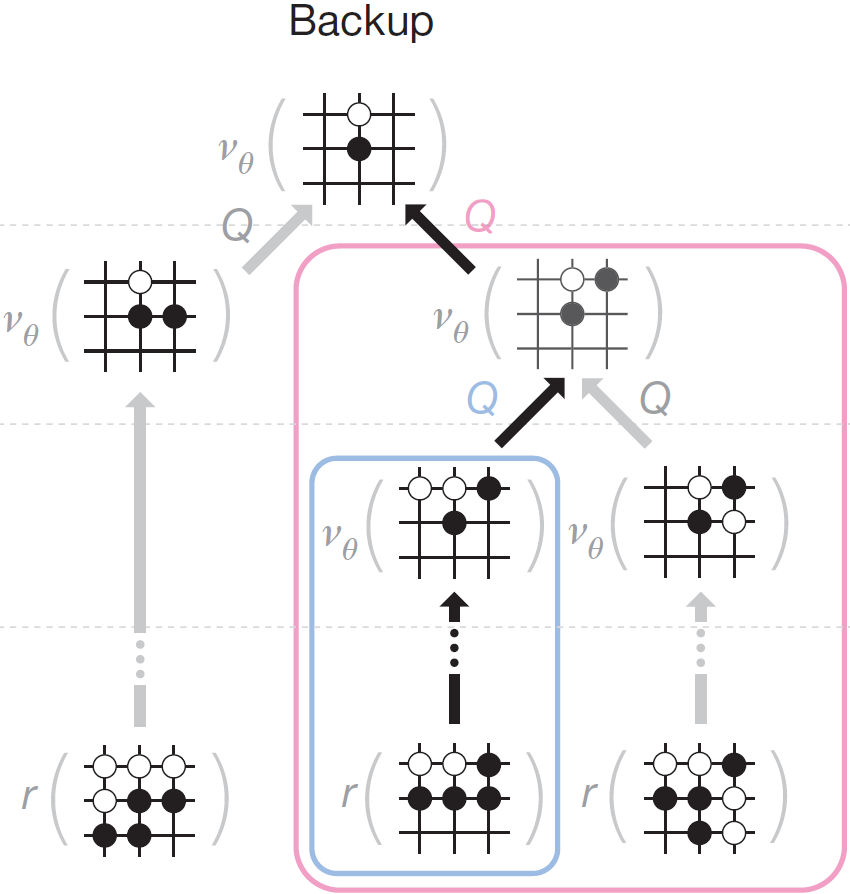
\includegraphics[height=.6\textheight]{../img/MCTS_backup.png}
      \end{center}
      
      At the end of a~simulation, each traversed edge \textbf{updates} its values.
    \end{frame}

    \begin{frame}[standout]
      Once the search is complete, the algorithm chooses \alert{the most visited move} from the root position.
    \end{frame}

    \begin{frame}{Tree Evaluation: using Value Network}
      \begin{center}
        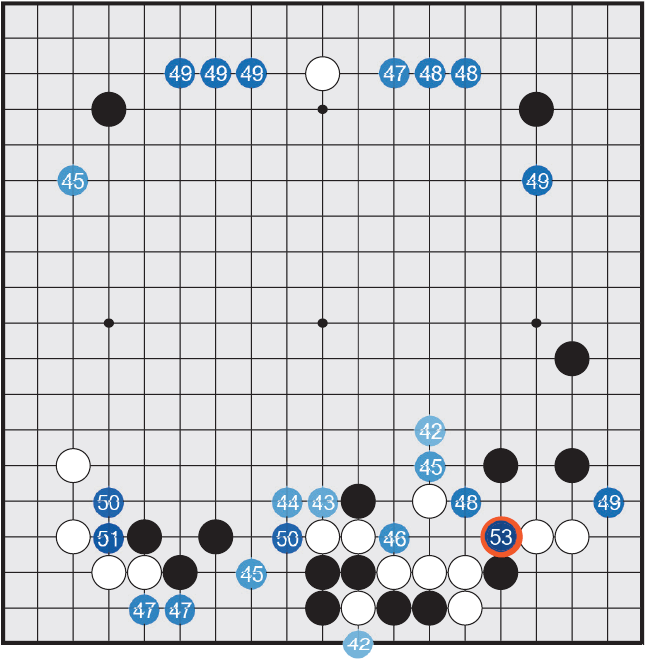
\includegraphics[height=.82\textheight]{../img/tree_eval_from_value_network.png}

        \tiny
        tree-edge values averaged over value network evaluations only
      \end{center}
    \end{frame}

    \begin{frame}{Tree Evaluation: using Rollouts}
      \begin{center}
        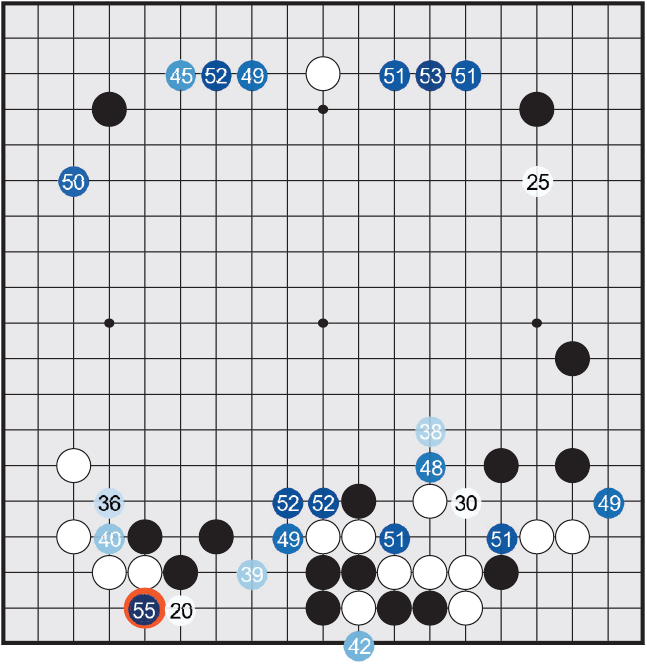
\includegraphics[height=.82\textheight]{../img/tree_eval_from_rollouts.png}

        \tiny
        tree-edge values averaged over rollout evaluations only
      \end{center}
    \end{frame}

    \begin{frame}{Percentage of~Simulations}
      \begin{center}
        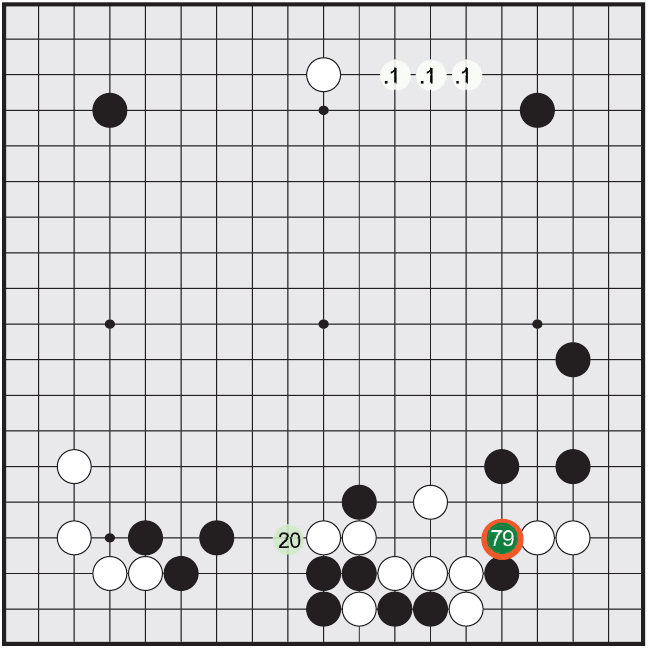
\includegraphics[height=.8\textheight]{../img/percentage_of_simulations.png}

        \tiny
        percentage frequency:\\
        which actions were selected during simulations
      \end{center}
    \end{frame}

    \begin{frame}{Principal Variation \\
        \tiny i.e. the Path with the Maximum Visit Count}
      \begin{center}
        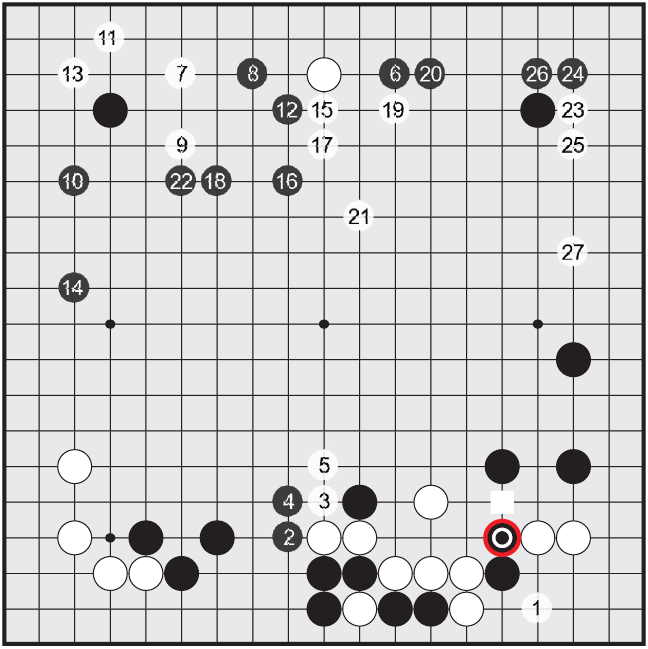
\includegraphics[height=.65\textheight]{../img/principal_variation.png}
      \end{center}
      \pause

      \vskip -1ex
      \begin{tiny}
        \begin{itemize}[<+- | alert@+>]
          \item AlphaGo selected the move indicated by the red circle.
          \item Fan Hui responded with the move indicated by the white square.
          \item In his post-game commentary, he preferred the move predicted by AlphaGo (label 1).
        \end{itemize}
      \end{tiny}
      \vskip 1.45em
    \end{frame}

    \begin{frame}{Tournament with Other Go Programs}
      \begin{center}
        \vskip -1ex
        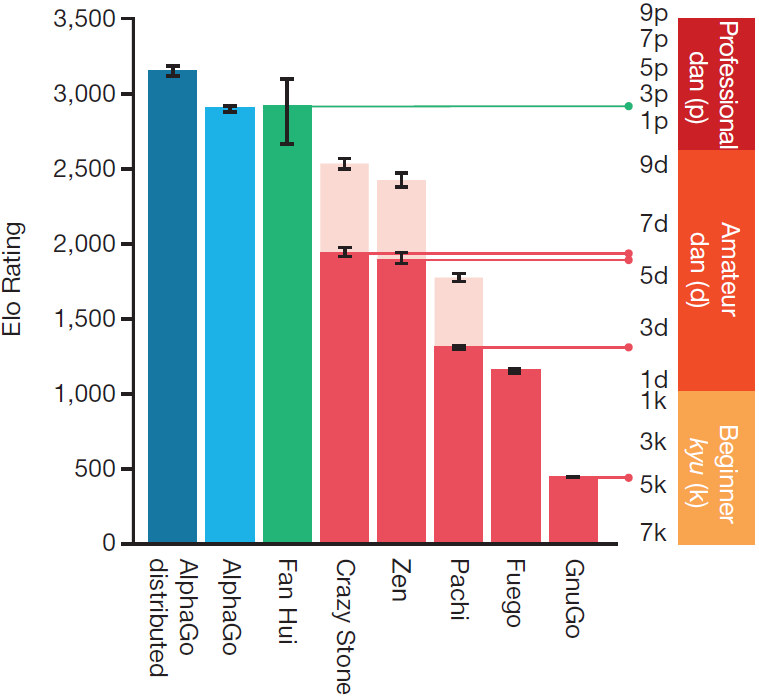
\includegraphics[height=.95\textheight]{../img/results_of_tournament.png}
      \end{center}
    \end{frame}
  }

  {
    \setbeamertemplate{frame footer}{\url{https://en.wikipedia.org/wiki/Fan_Hui}}
    \begin{frame}{Fan Hui}
      \begin{center}
        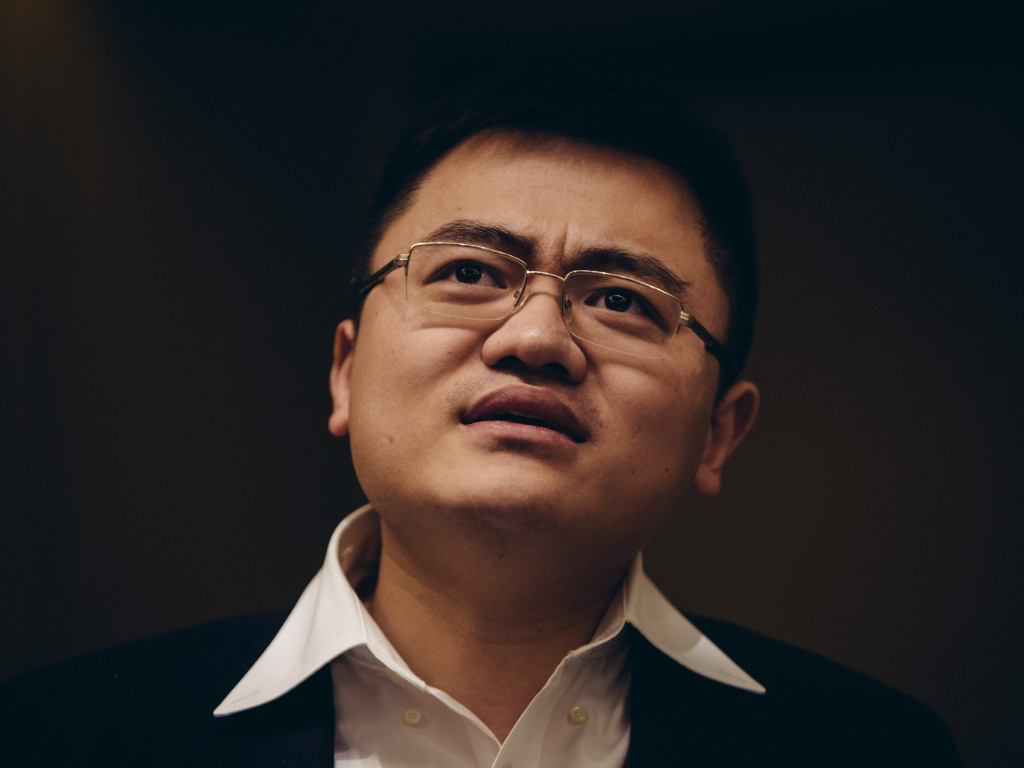
\includegraphics[width=.55\textwidth]{../img/Fan_Hui_profile.jpg}
      \end{center}
      \pause
      \vskip -1.6em
      \begin{itemize}[<+- | alert@+>]
        \item professional 2 dan
        \item European Go Champion in 2013, 2014 and 2015
        \item European Professional Go Champion in 2016 
        \item biological neural network:
          \begin{itemize}[<+- | alert@+>]
            \item 100 billion neurons
            \item 100 up to 1,000 trillion neuronal connections
          \end{itemize}
      \end{itemize}
    \end{frame}
  }

  \begin{frame}{AlphaGo versus Fan Hui}
    \pause
    \begin{center}
      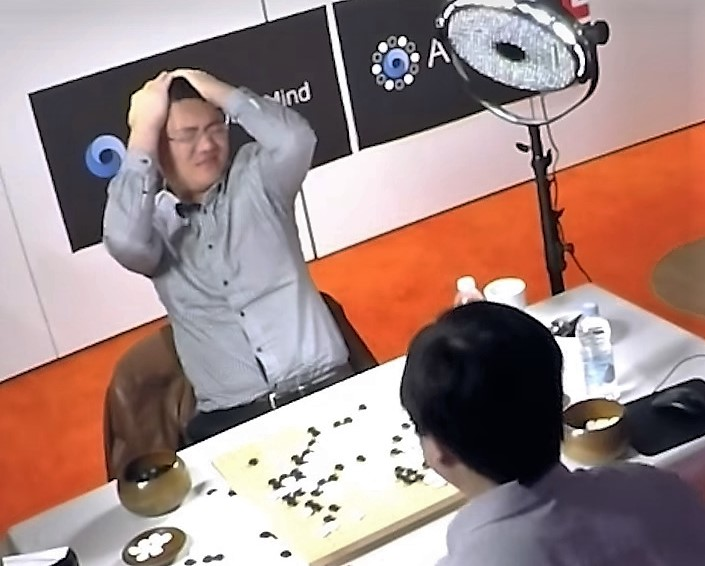
\includegraphics[width=.55\textwidth]{../img/Fan_Hui_loses.jpg}
    \end{center}
    \textbf{AlphaGo won 5 - 0} in a~formal match on~October 2015.
    \pause

    \vskip -1em
    \epigraph{
      \tiny
      [AlphaGo] is very strong and stable, it seems like a~wall.
      ...
      I know AlphaGo is a~computer, but if no one told me, maybe I would think the player was a~little strange, but a~very strong player, a~real person.
    }{Fan Hui}
  \end{frame}

  {
    \setbeamertemplate{frame footer}{\url{https://en.wikipedia.org/wiki/Lee_Sedol}}
    \begin{frame}{Lee Sedol ``The Strong Stone''}
      \begin{center}
        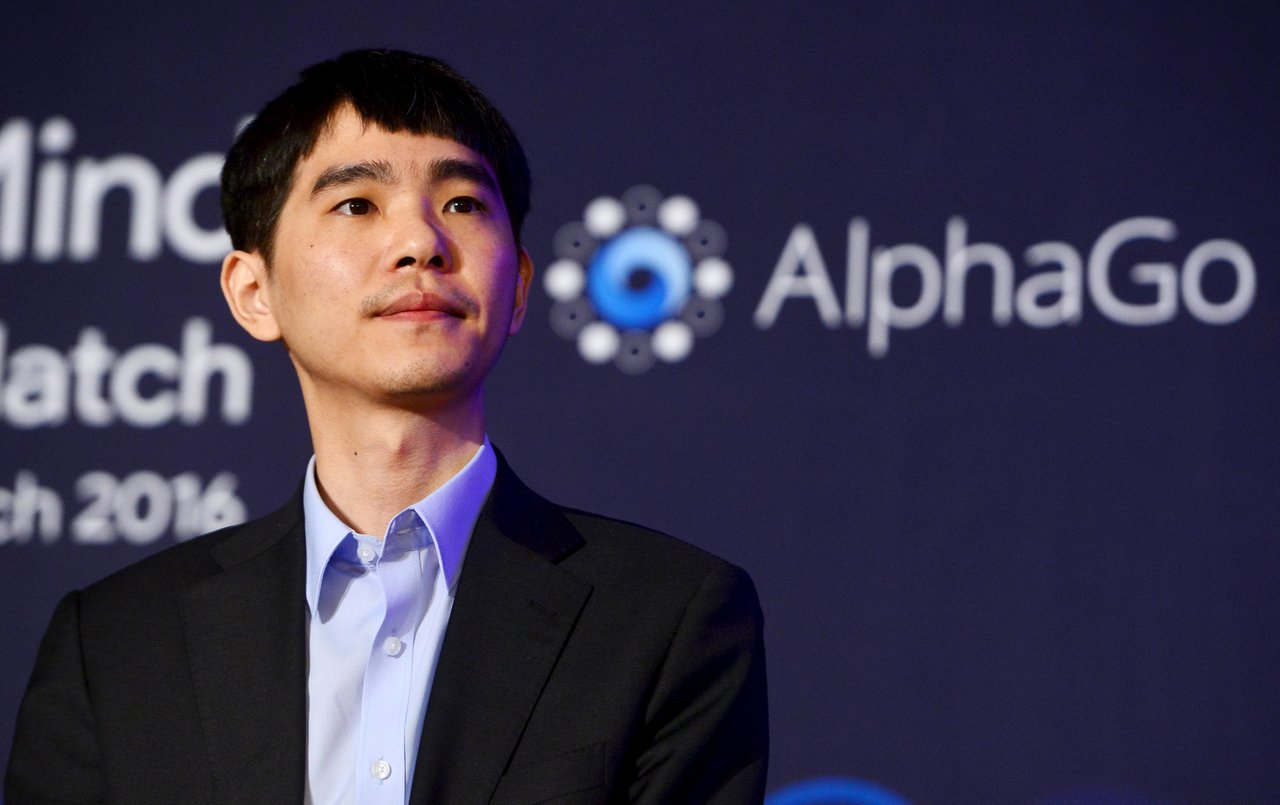
\includegraphics[width=.55\textwidth]{../img/Lee_Sedol_profile.jpg}
      \end{center}
      \pause
      \vskip -1.6em
      \begin{itemize}[<+- | alert@+>]
        \item professional 9 dan
        \item the $2^{nd}$ in international titles
        \item the $5^{th}$ youngest (12 years 4 months) to become a~professional Go player in~South Korean history
        \item Lee Sedol would win 97 out of~100 games against Fan Hui.
        \item biological neural network, comparable to Fan Hui's (in~number of~neurons and connections)
      \end{itemize}
    \end{frame}
  }

  {
    \usebackgroundtemplate{
      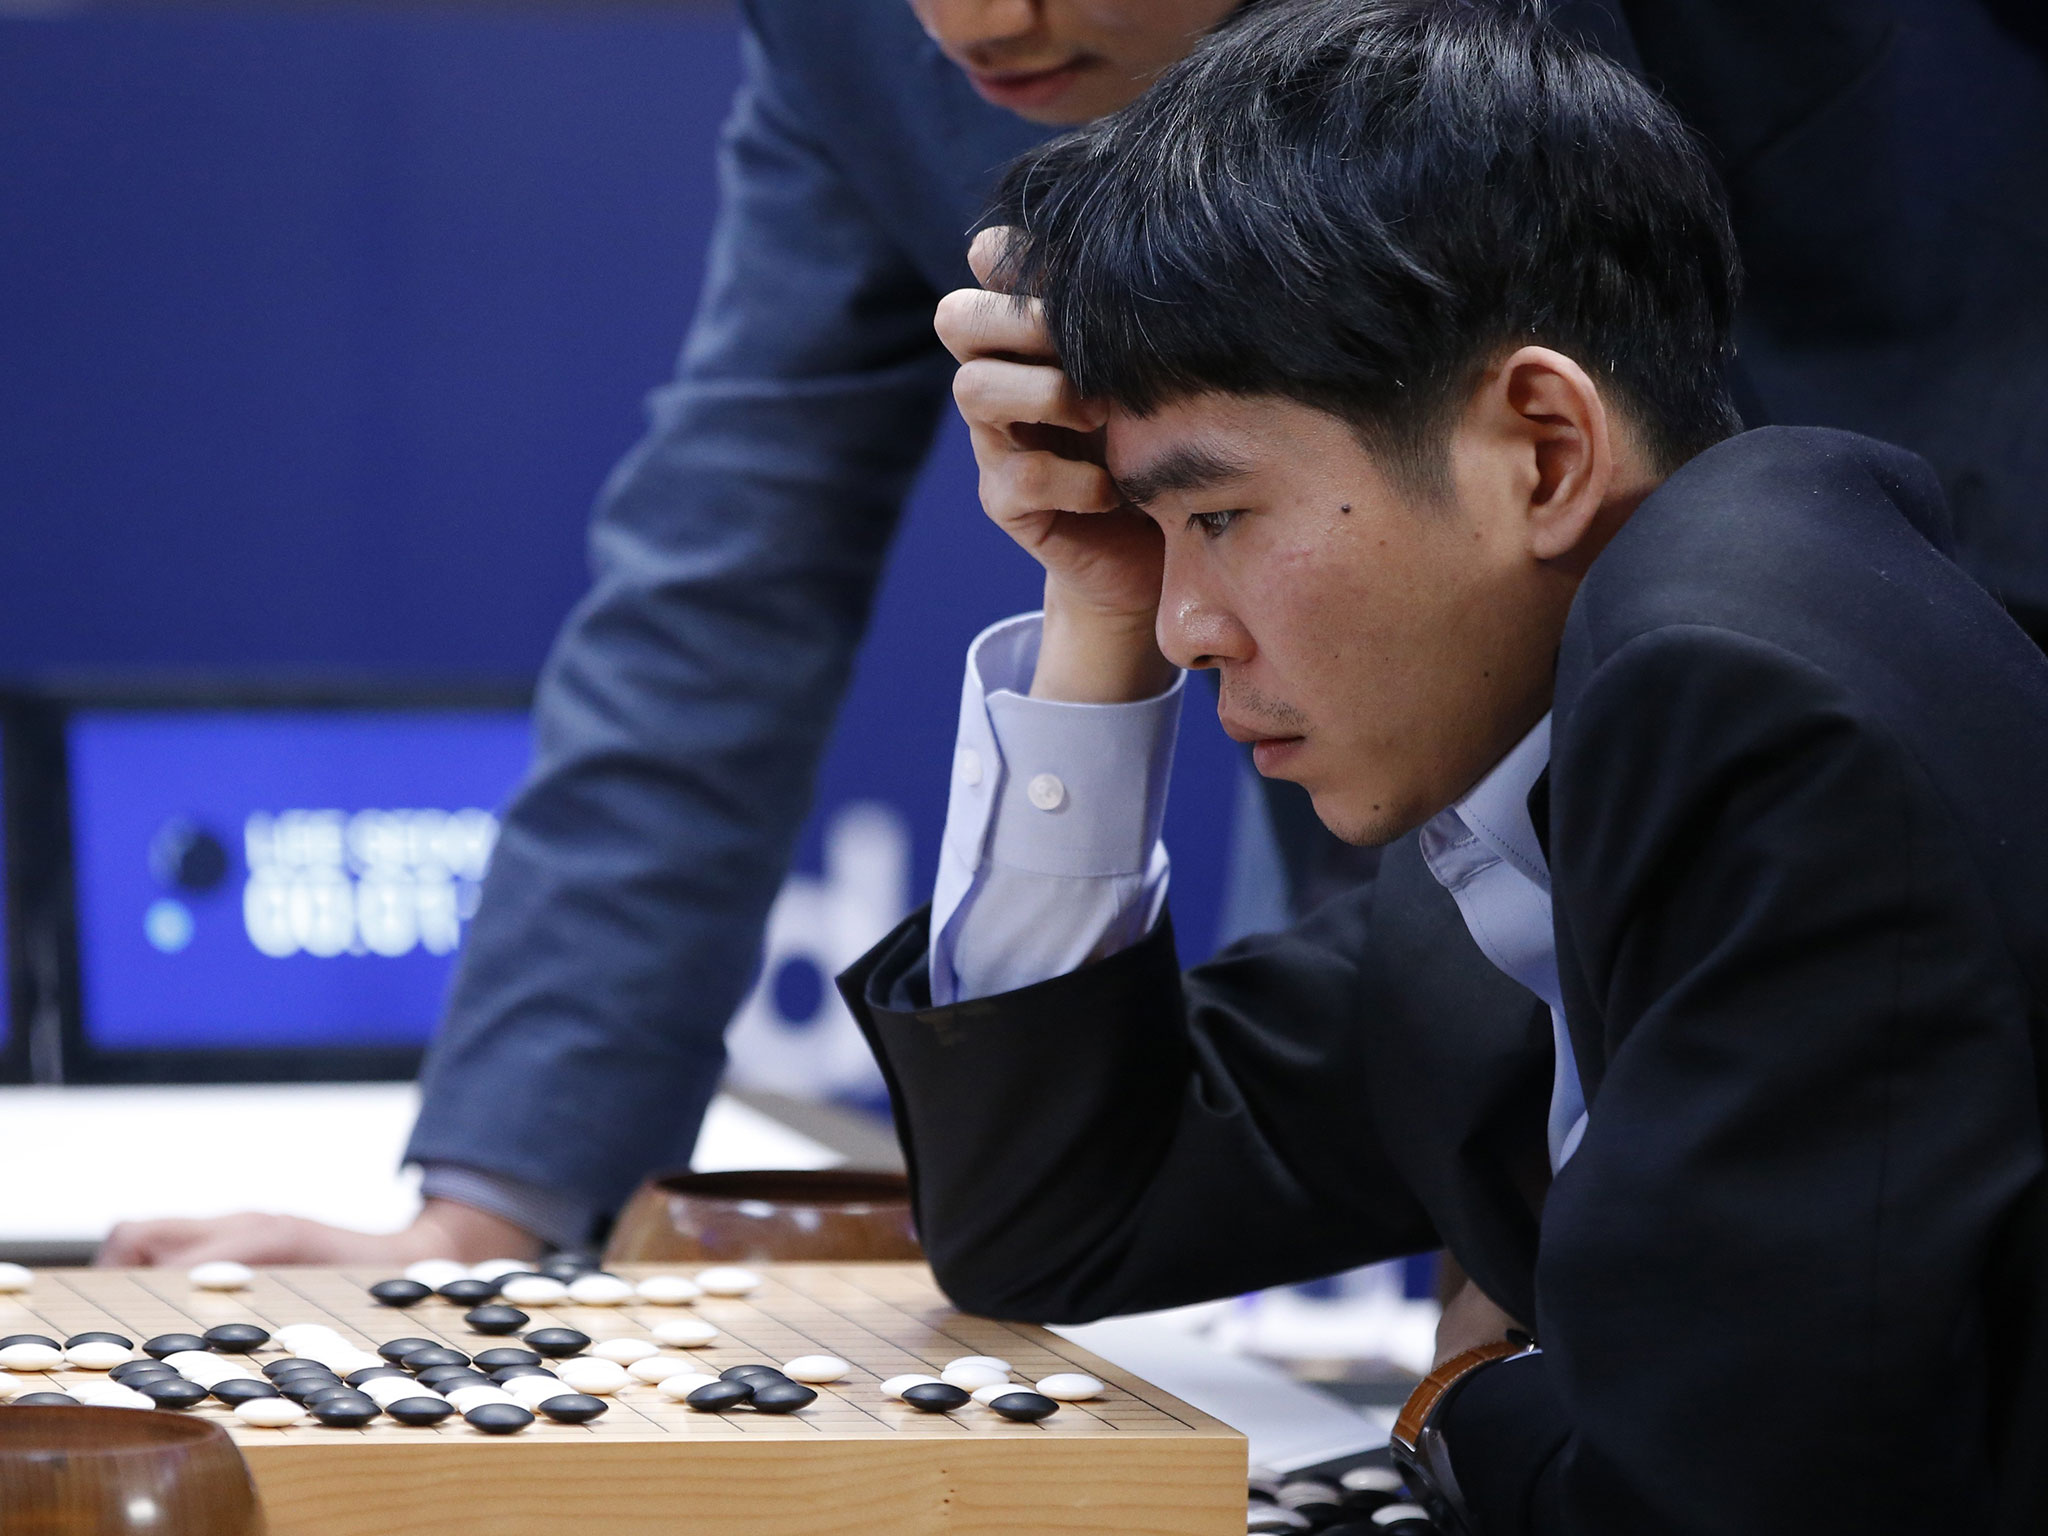
\includegraphics[height=\paperheight]{../img/Lee_Sedol_quotes.jpg}
    }
    \begin{frame}[standout]
      \epigraph{
        \tiny
        I heard Google DeepMind's AI is surprisingly strong and getting stronger, but I am confident that I can win, at least this time.
      }{Lee Sedol}
      \pause

      \epigraph{
        \tiny
        ...even beating AlphaGo by 4-1 may allow the Google DeepMind team to claim its de facto victory and the defeat of him [Lee~Sedol], or even humankind.
      }{interview in JTBC Newsroom}
      \pause
    \end{frame}
  }

  {
    \usebackgroundtemplate{
      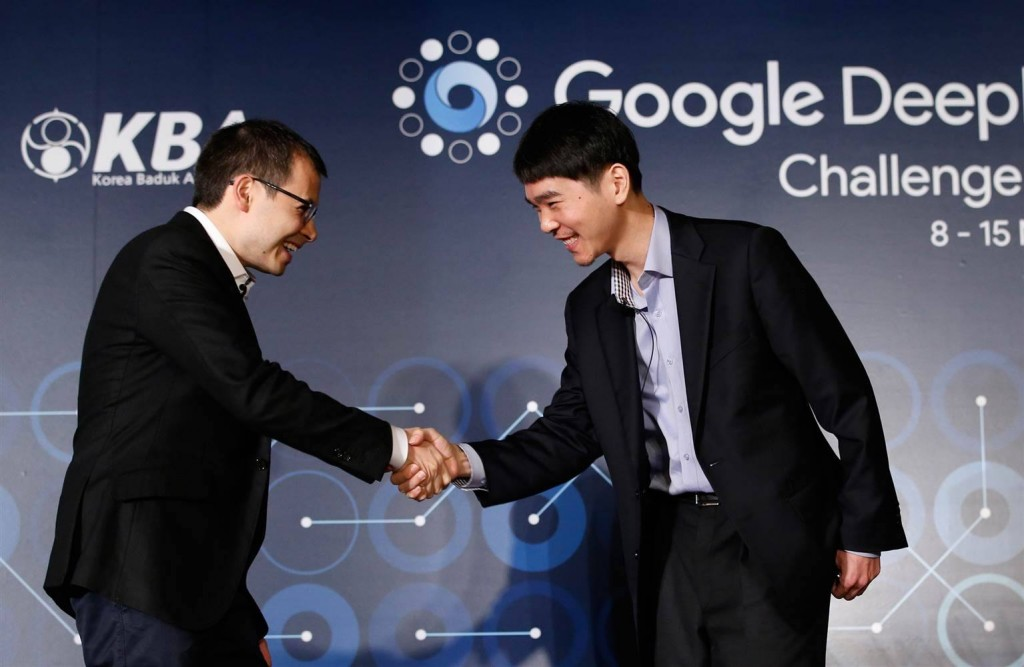
\includegraphics[height=\paperheight]{../img/Lee_Sedol_after_match.jpg}
    }
    \setbeamertemplate{frame footer}{\color{white}\url{https://en.wikipedia.org/wiki/AlphaGo_versus_Lee_Sedol}}
    \begin{frame}{AlphaGo versus Lee Sedol}
      \pause

      \vskip 1em
      \color{white}
      In March 2016 AlphaGo won 4-1 against the legendary Lee Sedol.
      \pause

      \textbf{AlphaGo won all but the $4^{th}$ game; all games were won by~resignation.}
      \pause

      \textbf{The winner of~the match was slated to win \$1 million.}
      \pause

      \textbf{Since AlphaGo won, Google DeepMind stated that the prize will be donated to~charities, including~UNICEF, and Go organisations.}
      \pause

      \textbf{Lee received \$170,000 (\$150,000 for participating in all the five games, and an additional \$20,000 for each game won).}
    \end{frame}
  }

%%%%%%%%%%%%%%%%%%%%%%%%%%%%%%%%%%%%%%%%%%%%%%%%%%%%%%%%%%%%%%%%%%%%%%%%%%%%%%%%

  \section{Poker: Cepheus, DeepStack}

  {
    \usebackgroundtemplate{
      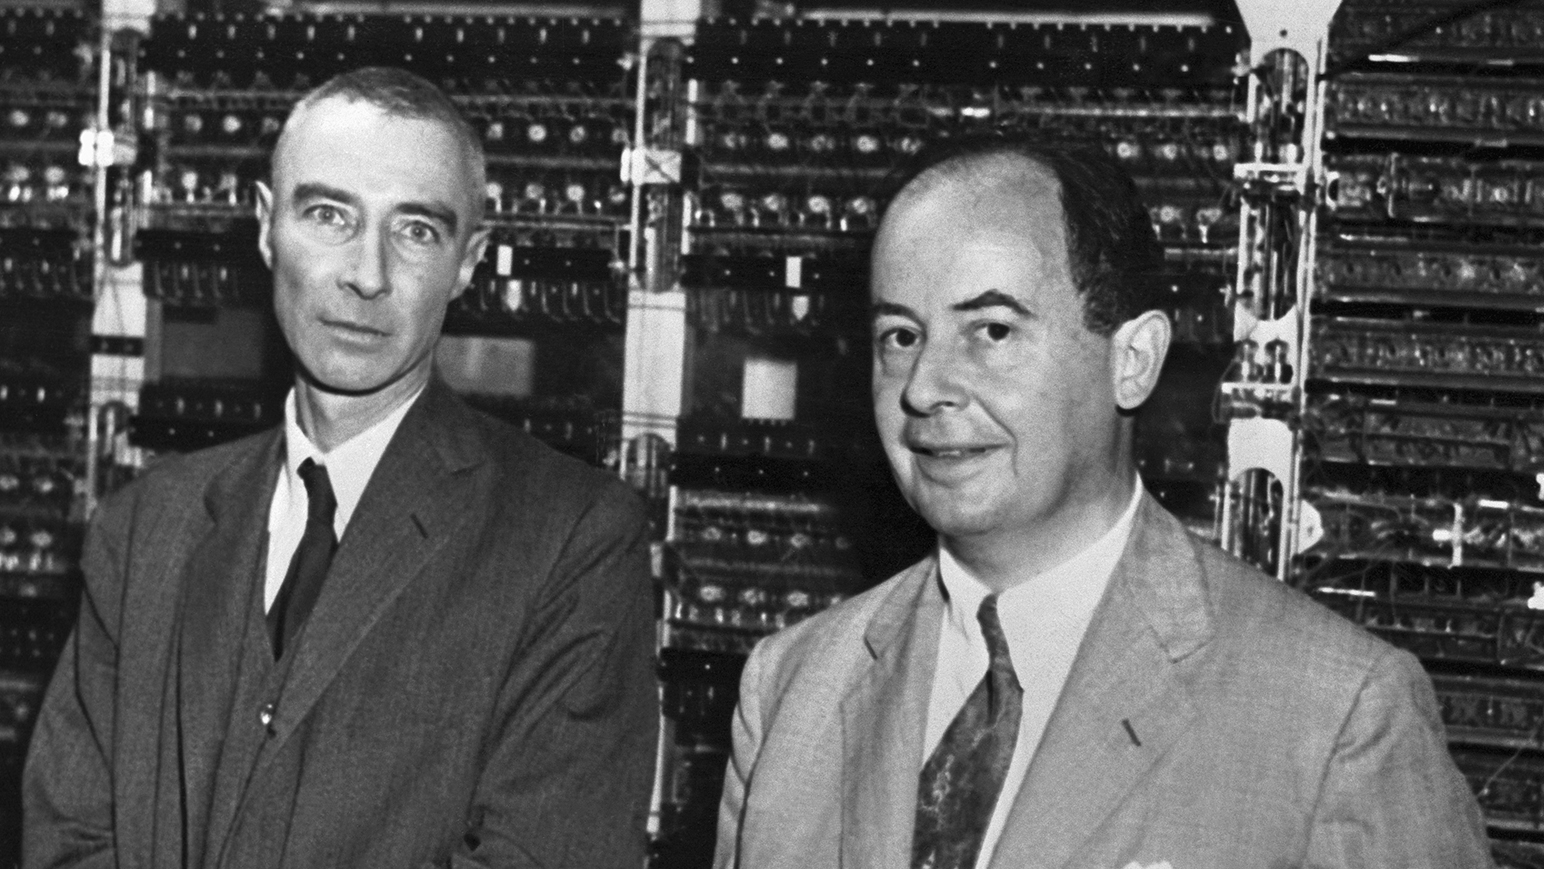
\includegraphics[width=\paperwidth]{../img/john-von-neumann-p-cropped.jpg}
    }
    \begin{frame}[standout]
      \vskip 0.75\paperheight
      \color{black}
      \epigraph{
        \tiny
        Real life consists of bluffing, of little tactics of deception, of asking yourself what is the other man going to think I mean to do.
      }{John von Neumann}
    \end{frame}
  }

  {
    \setbeamertemplate{frame footer}{\deepStackCitation}
    \begin{frame}{Game Tree in Poker}
      \begin{center}
        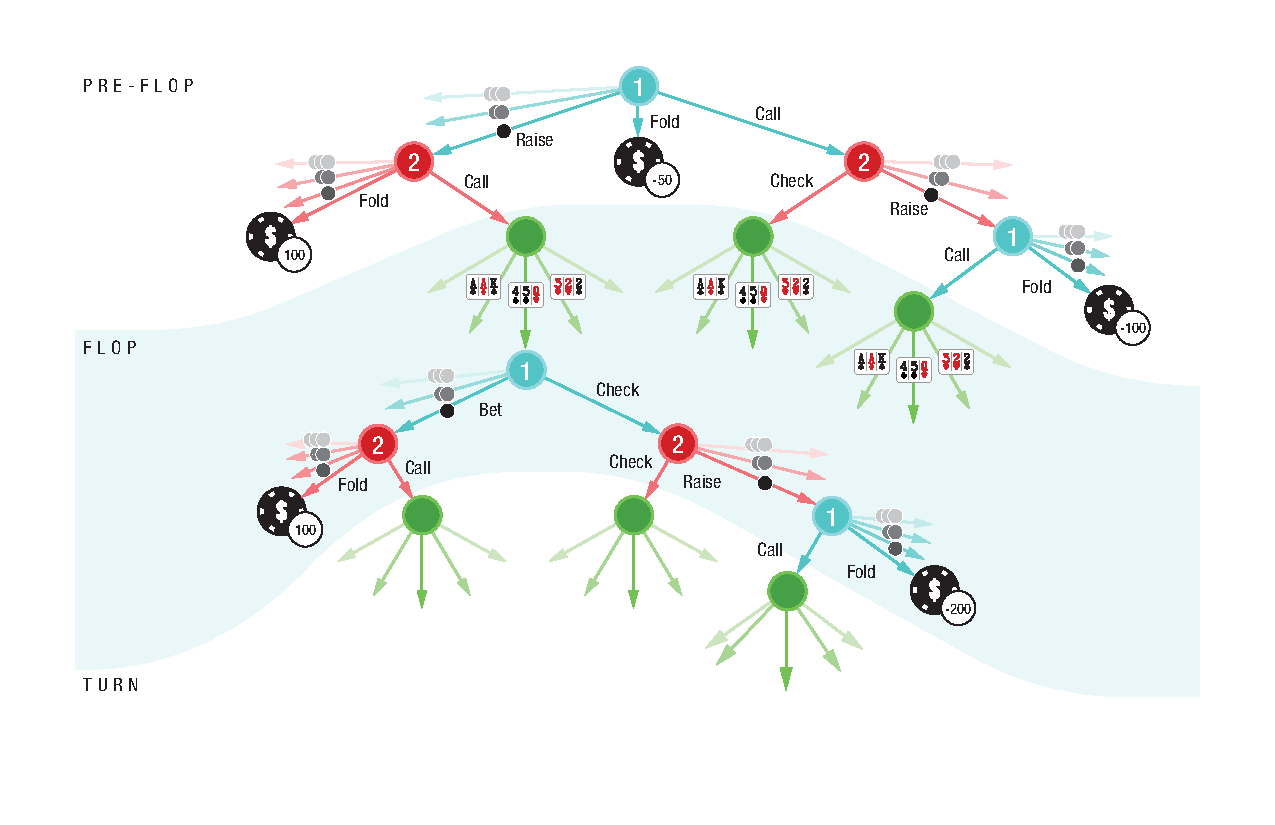
\includegraphics[width=\textwidth, keepaspectratio]{../img/public_tree.pdf}
      \end{center}
      \pause
      \begin{center}
        the so-called \textbf{public tree} (tree of public events)
      \end{center}
    \end{frame}
  }

  \begin{frame}[standout]
    \begin{center}
      Cepheus
    \end{center}
  \end{frame}

  {
    \setbeamertemplate{frame footer}{\cepheusCitation}
    \begin{frame}{Cepheus\\
        \tiny Heads-up Limit Hold’em Poker}
      \pause
      \begin{center}
        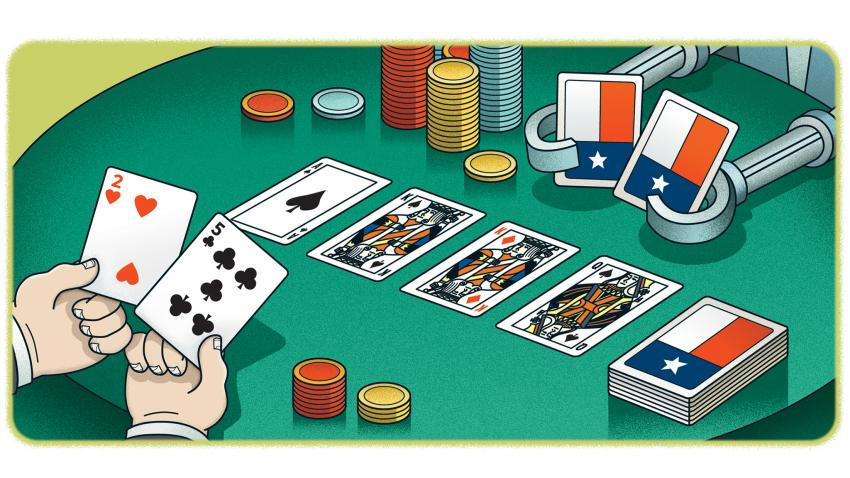
\includegraphics[width=\textwidth, keepaspectratio]{../img/limit_holdem_poker.jpg}

        \url{http://poker.srv.ualberta.ca/}
      \end{center}
    \end{frame}
  }

  \begin{frame}[standout]
    \begin{center}
      DeepStack
    \end{center}
  \end{frame}

  {
    \usebackgroundtemplate{
      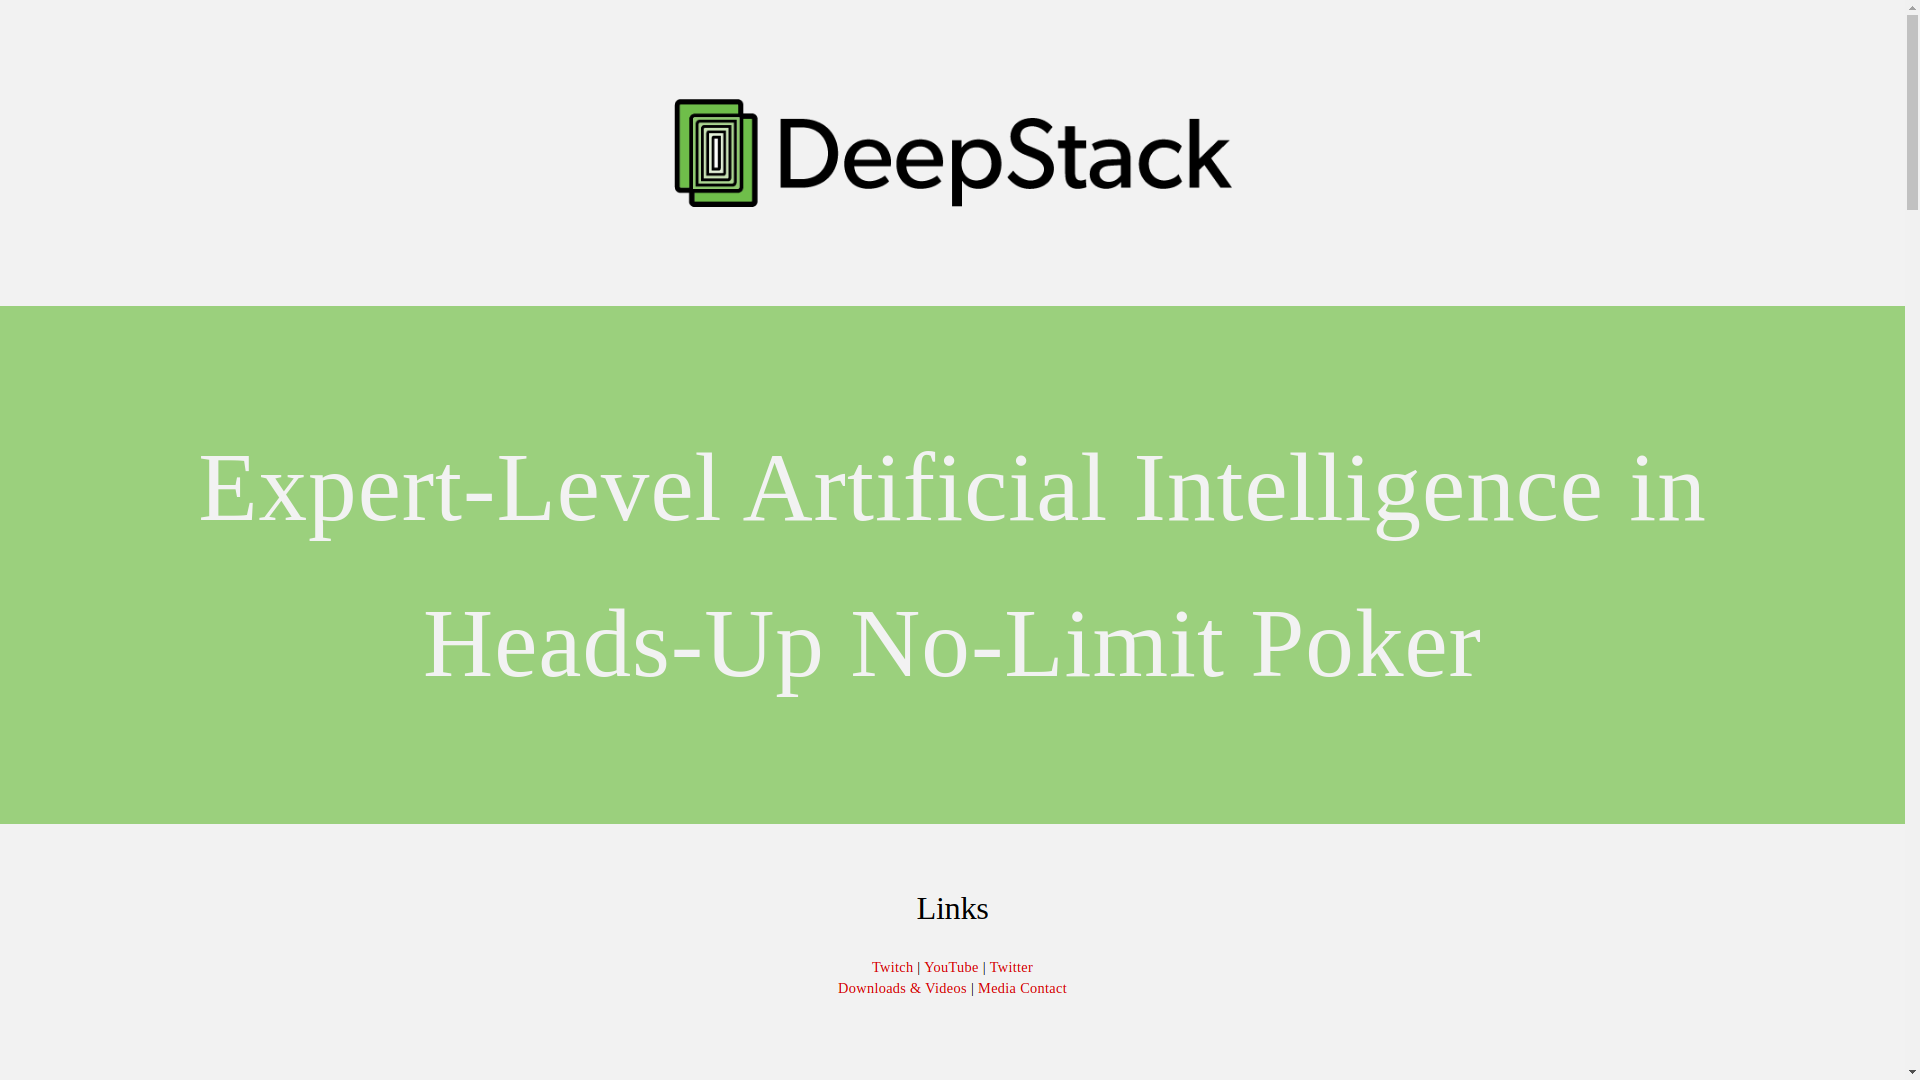
\includegraphics[width=\paperwidth]{../img/deepstack_ai.png}
    }
    \begin{frame}[standout]
      \begin{center}
        \vskip 0.8\paperheight
        \color{black}
        \url{https://www.deepstack.ai}
      \end{center}
    \end{frame}
  }

  {
    \setbeamertemplate{frame footer}{\deepstackAiCitation}
    \begin{frame}{DeepStack}
      \begin{center}
        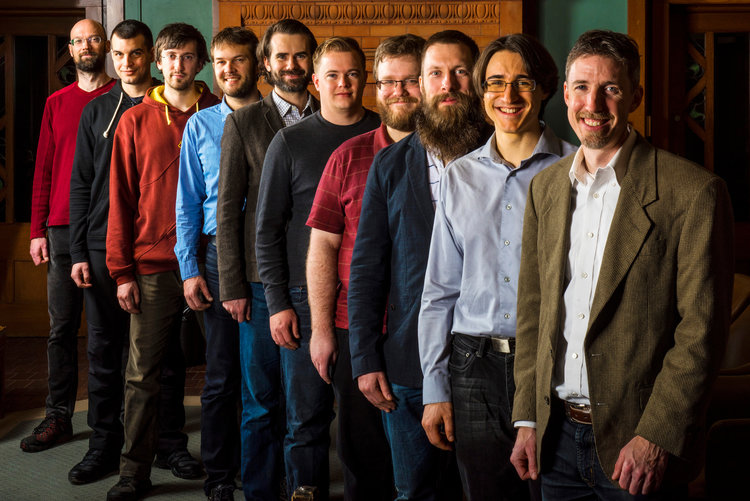
\includegraphics[height=.6\textheight]{../img/DeepStackResearchers.jpg}
      \end{center}
      \pause
      \vskip -1.5em
      \begin{itemize}[<+- | alert@+>]
        \item completed in December 2016
        \item published in Science in March 2017
        \item the first AI capable of beating (11) professional poker players
        \item 44,000 hands of \textbf{Heads-Up No-Limit Texas Hold'em}
      \end{itemize}
    \end{frame}
  }

  {
    \setbeamertemplate{frame footer}{\deepStackCitation}
    \begin{frame}{DeepStack: Components}
      \begin{center}
        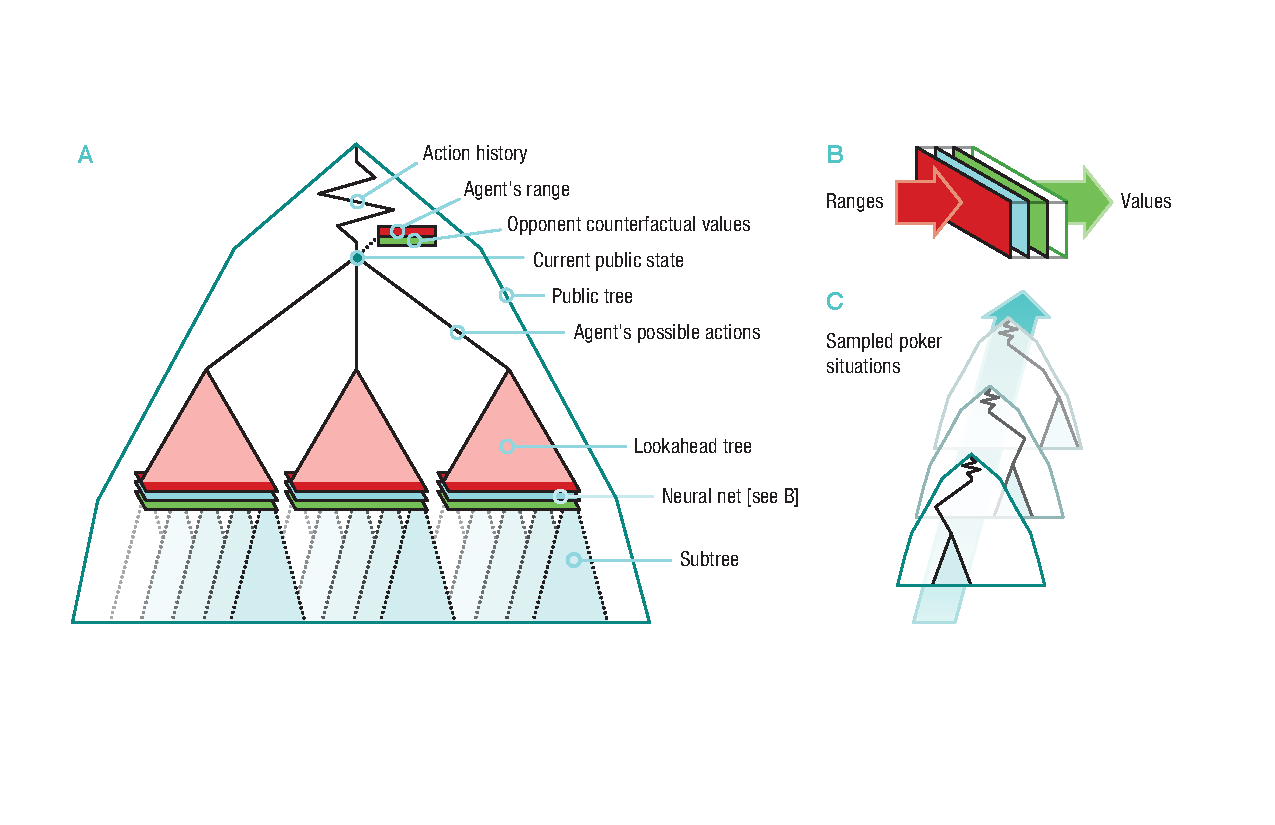
\includegraphics[width=\textwidth, keepaspectratio]{../img/taking_actions.pdf}
      \end{center}
      \pause
      \begin{itemize}[<+- | alert@+>]
        \item continual resolving
        \item ``intuitive'' local search
        \item sparse lookahead trees
      \end{itemize}
    \end{frame}
  }

  {
    \setbeamertemplate{frame footer}{\deepstackAiCitation}
    \begin{frame}{DeepStack: Continual Resolving}
      \begin{center}
        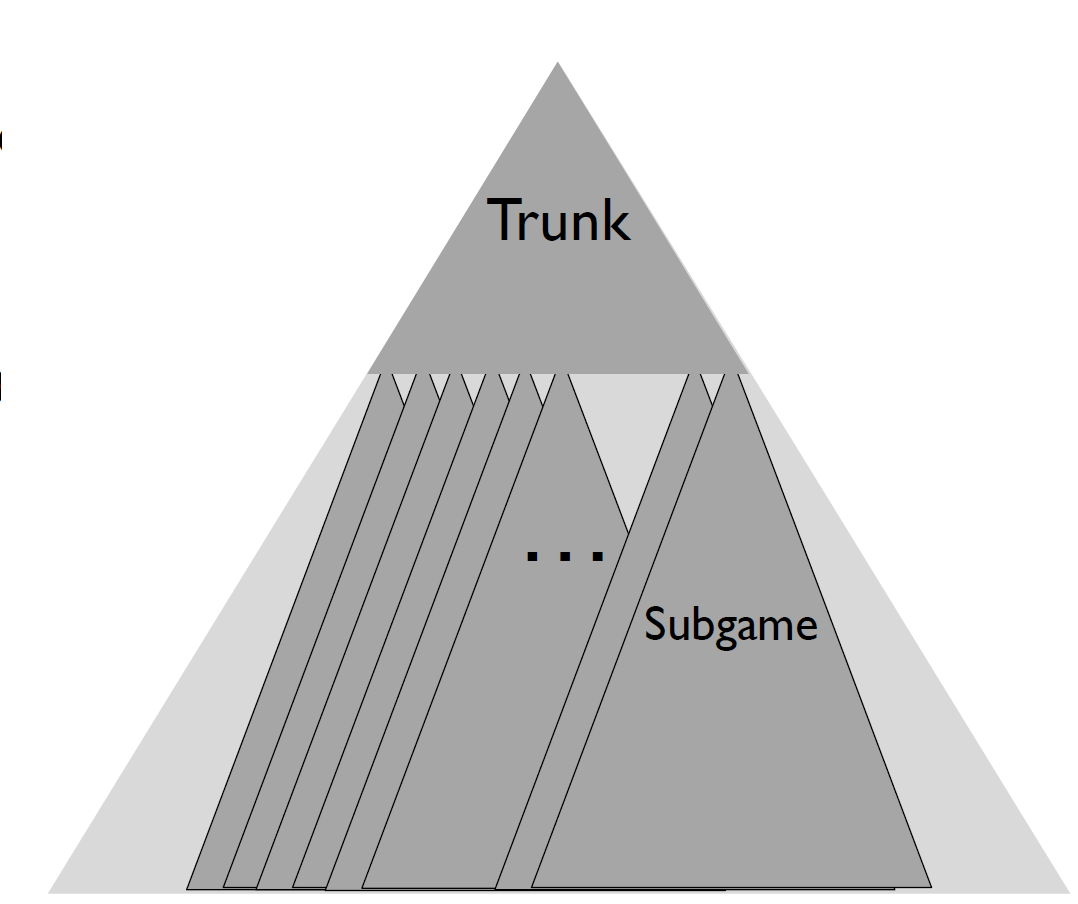
\includegraphics[height=0.55\textheight, width=\textwidth, keepaspectratio]{../img/subgames-cfr-d.png}
      \end{center}
      \pause
      \begin{itemize}[<+- | alert@+>]
        \item only a strategy based on the current state
        \item only for the remainder of the hand
        \item no strategy for the full game
        \item $\Rightarrow$ lower overall exploitability
      \end{itemize}
    \end{frame}

    \begin{frame}{DeepStack: ``Intuitive'' Local Search}
      \begin{itemize}[<+- | alert@+>]
        \item no reasoning about the full remaining game
        \item computation beyond a certain depth: a fast-approximate estimate
        \item namely, deep neural networks
        \item ``gut feeling'' of the value of holding any cards in any situation
      \end{itemize}
      \pause
    \end{frame}
  }

  {
    \setbeamertemplate{frame footer}{\deepStackCitation}
    \begin{frame}{DeepStack: Deep Counterfactual Value Network}
      \begin{center}
        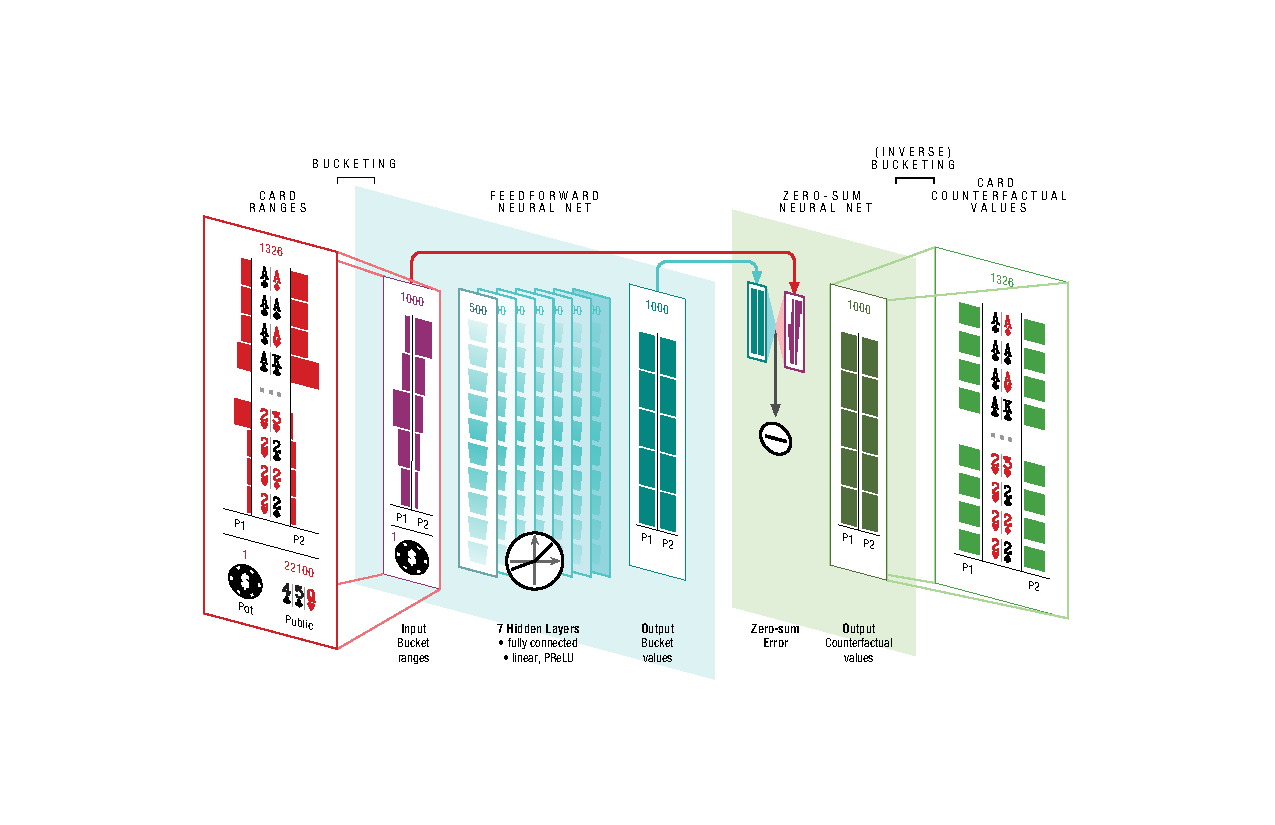
\includegraphics[width=\textwidth, keepaspectratio]{../img/dnn.pdf}
      \end{center}
    \end{frame}
  }

  {
    \setbeamertemplate{frame footer}{\deepstackAiCitation}
    \begin{frame}{DeepStack: Sparse Lookahead Trees}
      \begin{itemize}[<+- | alert@+>]
        \item a reduced number of actions considered
        \item to play at conventional human speeds
        \item games re-solved in under five seconds
        \item on a simple gaming laptop
        \item with an NVIDIA GeForce GTX 1080 GPU
      \end{itemize}
    \end{frame}
  }

  {
    \setbeamertemplate{frame footer}{\deepStackCitation}
    \begin{frame}{DeepStack: Against Professional Players}
      \begin{center}
        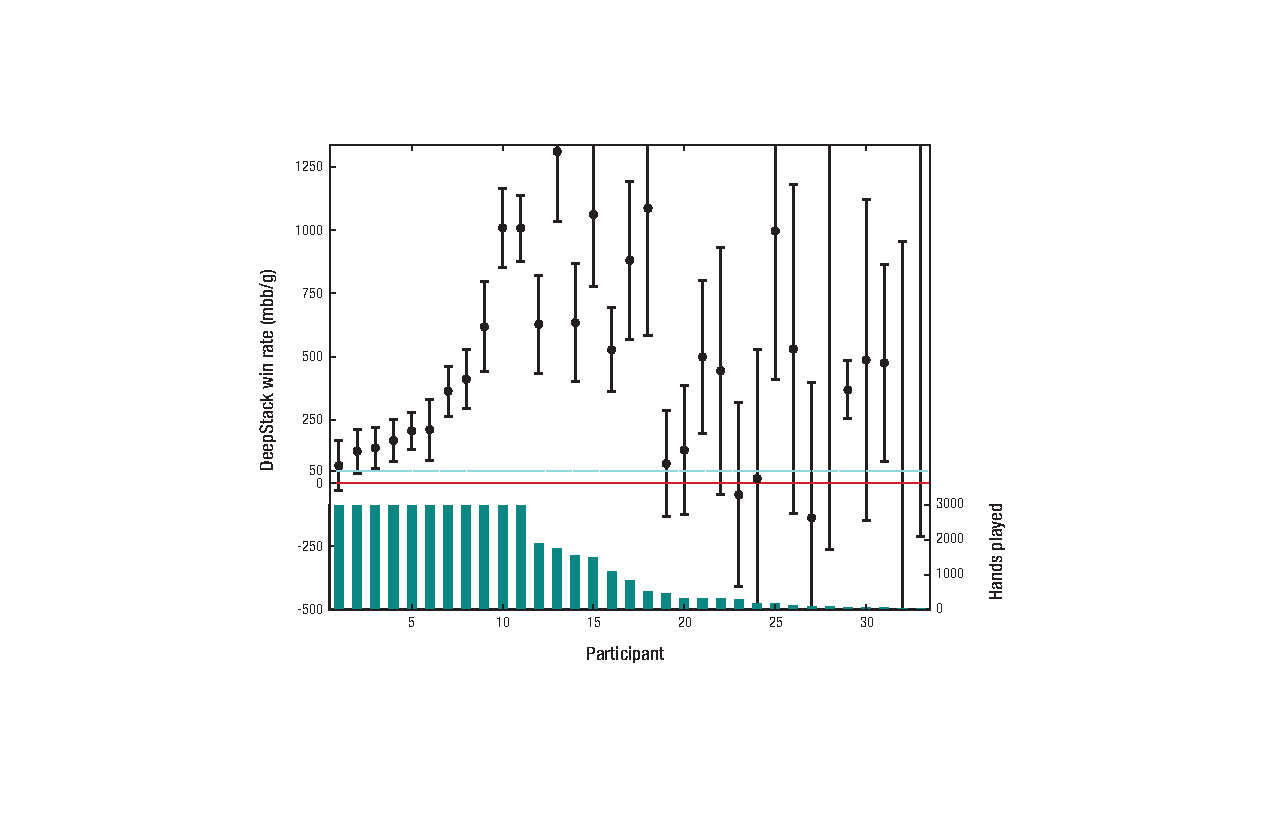
\includegraphics[width=\textwidth, keepaspectratio]{../img/humans_curio.pdf}
      \end{center}
    \end{frame}

    \begin{frame}{DeepStack: Theoretical Guarantees}
      \begin{theorem}
        \begin{itemize}[<+- | alert@+>]
          \item Let the error of \emph{counterfactual values} returned by the value function be $\le\epsilon$.
          \item Let $T$ be the number of resolving iterations for each decision.
        \end{itemize}
        \pause
        Then the exploitability of~the strategies is
        \[
          \le k_1 \epsilon + \frac{k_2}{\sqrt{T}}
        \]
        where $k_1$ and $k_2$ are game-specific constants.
      \end{theorem}
    \end{frame}
  }

%%%%%%%%%%%%%%%%%%%%%%%%%%%%%%%%%%%%%%%%%%%%%%%%%%%%%%%%%%%%%%%%%%%%%%%%%%%%%%%%

  \section{Beyond DeepStack: TensorCFR}

  {
    \usebackgroundtemplate{
      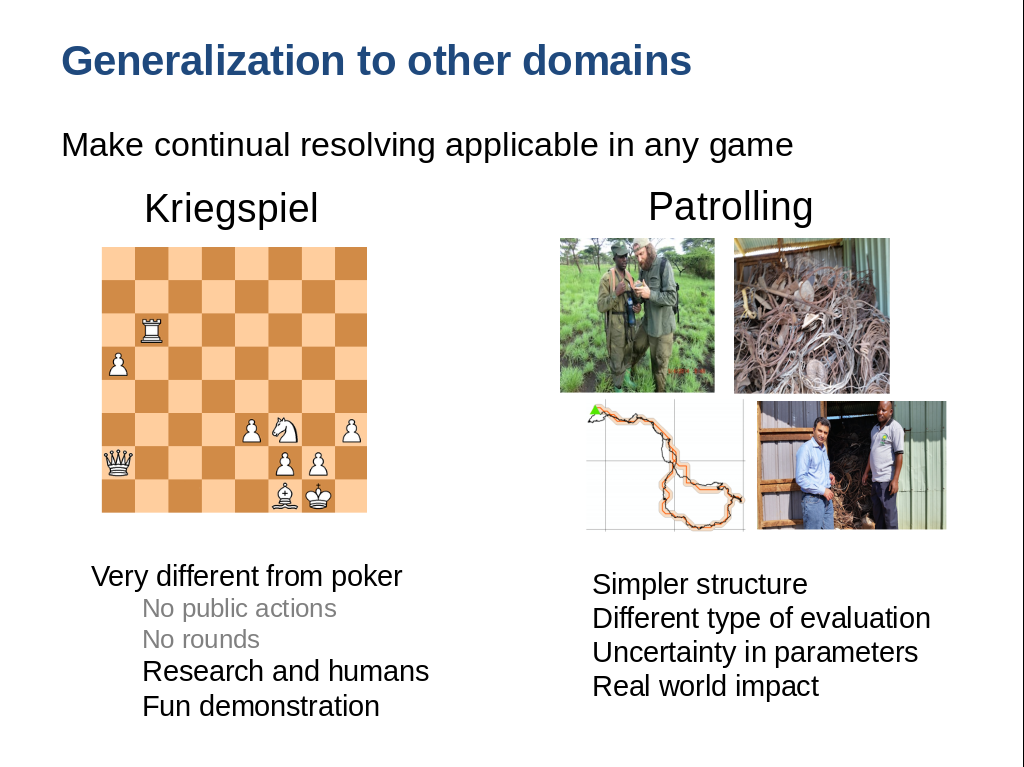
\includegraphics[width=\paperwidth, keepaspectratio]{../img/gacr-2018-generalization-to-other-domains.png}
    }
    \setbeamertemplate{frame footer}{\colorcite from presentation of dr. Viliam Lisý}
    \begin{frame}[standout]
    \end{frame}
  }

%%%%%%%%%%%%%%%%%%%%%%%%%%%%%%%%%%%%%%%%%%%%%%%%%%%%%%%%%%%%%%%%%%%%%%%%%%%%%%%%

  \section{Conclusion}

  \begin{frame}[standout]
    \begin{center}
      Thank you!

      Questions?
    \end{center}
  \end{frame}

%%%%%%%%%%%%%%%%%%%%%%%%%%%%%%%%%%%%%%%%%%%%%%%%%%%%%%%%%%%%%%%%%%%%%%%%%%%%%%%%

  \appendix
  \begin{frame}[standout]
    Backup Slides
  \end{frame}

  {
    \setbeamertemplate{frame footer}{\alphaGoCitation}
    \begin{frame}{SL Policy Networks (1/2)}
      \begin{itemize}[<+- | alert@+>]
        \item 13-layer deep convolutional neural network
        \item goal: to~predict expert human moves
        \item task of \textbf{classification}
        \item trained from 30 millions positions from the KGS Go Server
        \item stochastic gradient ascent:
          \[
            \Delta \sigma \propto \frac{\partial \log p_\sigma (a|s)}{\partial \sigma}
          \]
          {\tiny (to~maximize the likelihood of~the human move~$a$ selected in~state~$s$)}
      \end{itemize}
      \pause

      Results:
      \pause
      \begin{itemize}[<+- | alert@+>]
        \item $44.4\%$ accuracy (the state-of-the-art from other groups)
        \item $55.7\%$ accuracy (raw board position + move history as~input)
        \item $57.0\%$ accuracy (all input features)
      \end{itemize}
    \end{frame}

    \begin{frame}{SL Policy Networks (2/2)}
      Small improvements in~accuracy led to~large improvements in~playing strength (see the next slide)
      \begin{center}
        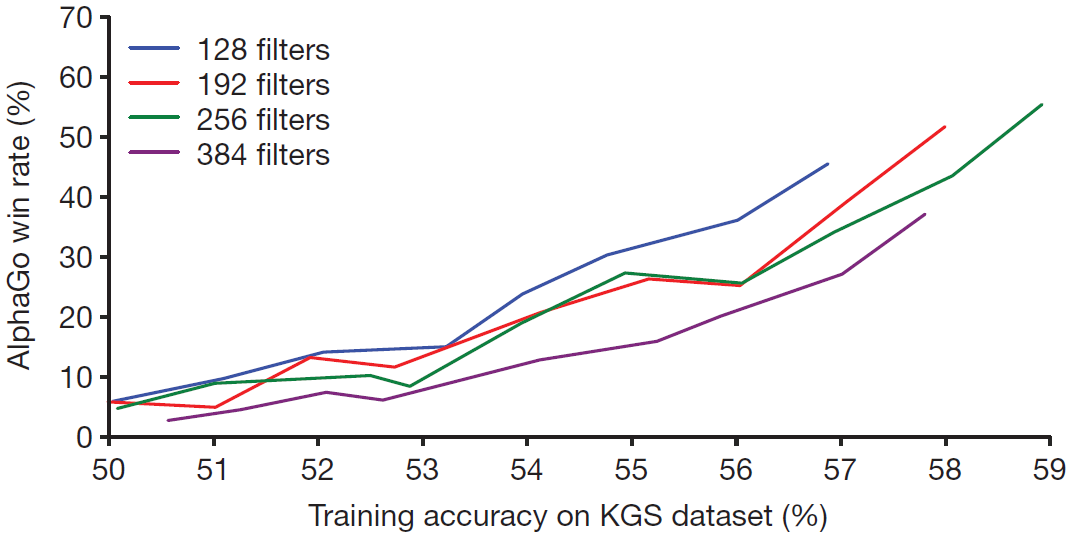
\includegraphics[width=\textwidth]{../img/SL_policy_accuracy_vs_win_rate.png}
      \end{center}
    \end{frame}

    \begin{frame}{RL Policy Networks (details)}
      Results (by sampling each move $a_t \sim p_\rho(\cdot | s_t)$):
      \pause
      \begin{itemize}[<+- | alert@+>]
        \item $80\%$ of~win rate against the SL policy network
        \item $85\%$ of~win rate against the strongest open-source Go program, \textbf{Pachi} (\cite{Baudivs2011pachi})
          \begin{itemize}[<+- | alert@+>]
            \item The previous state-of-the-art, based only on~SL of~CNN: \\
              \pause
              $11\%$ of~``win'' rate against Pachi
          \end{itemize}
      \end{itemize}
    \end{frame}

    \begin{frame}{Evaluation accuracy in~various stages of a~game}
      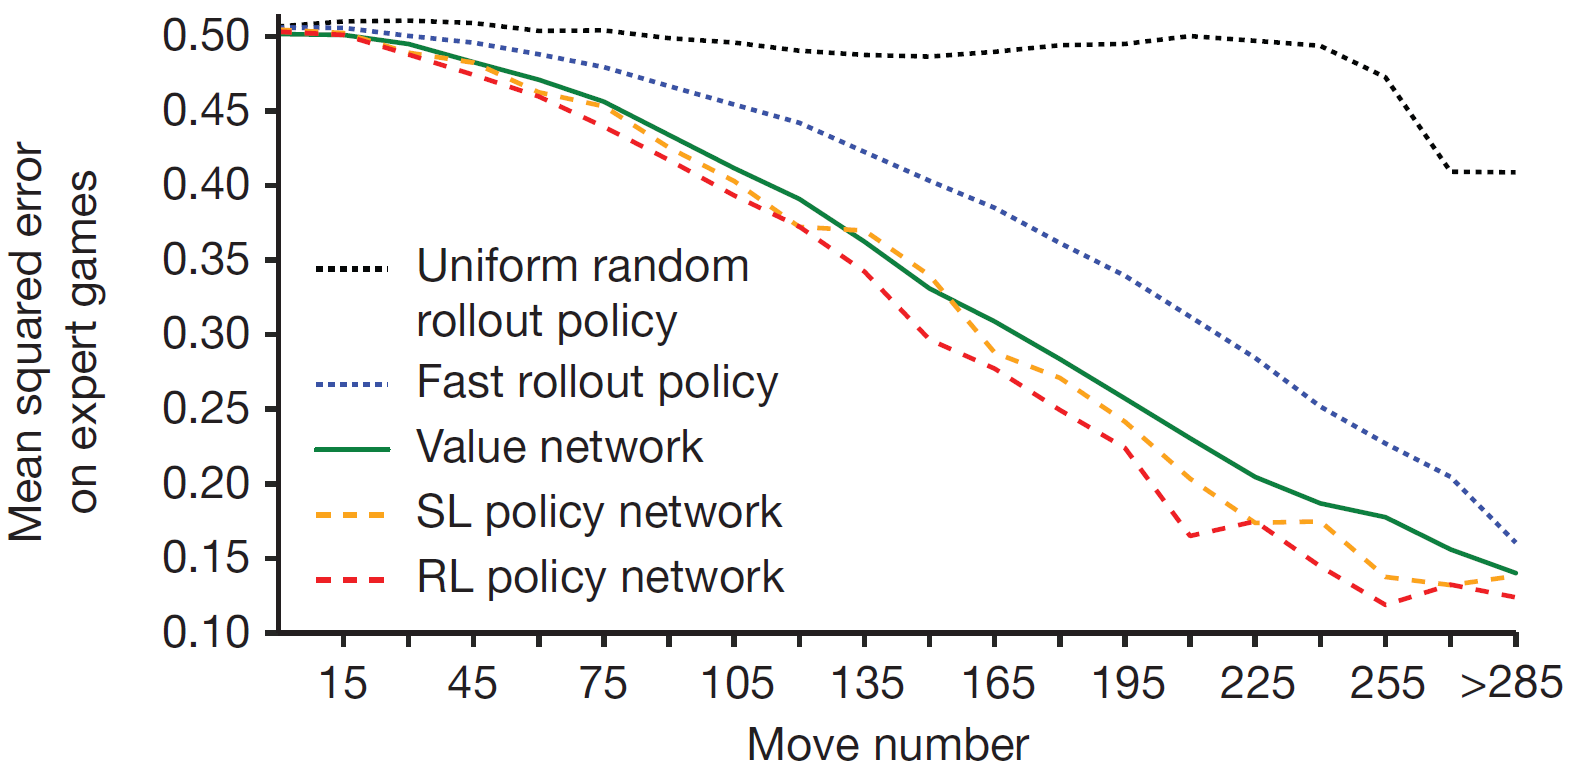
\includegraphics[width=\textwidth]{../img/policies_move_numbers_vs_MSE.png}

      \vskip -2.4ex
      {\tiny
      \textbf{Move number} is the number of~moves that had been played in the given position.
      }

      \pause
      Each position evaluated by:
      \begin{itemize}[<+- | alert@+>]
        \item forward pass of the value network~$v_\theta$
        \item 100 rollouts, played out using the corresponding policy
      \end{itemize}
    \end{frame}

    \begin{frame}{Scalability}
      \begin{itemize}
        \item asynchronous multi-threaded search
        \item simulations on~CPUs
        \item computation of~neural networks on GPUs
      \end{itemize}
      \pause

      AlphaGo:
      \begin{itemize}
        \item 40 search threads
        \item 40 CPUs
        \item 8 GPUs
      \end{itemize}
      \pause

      Distributed version of AlphaGo (on~multiple machines):
      \begin{itemize}
        \item 40 search threads
        \item 1202 CPUs
        \item 176 GPUs
      \end{itemize}
    \end{frame}

    \begin{frame}{ELO Ratings for~Various Combinations of~Threads}
      \begin{center}
        \vskip -1ex
        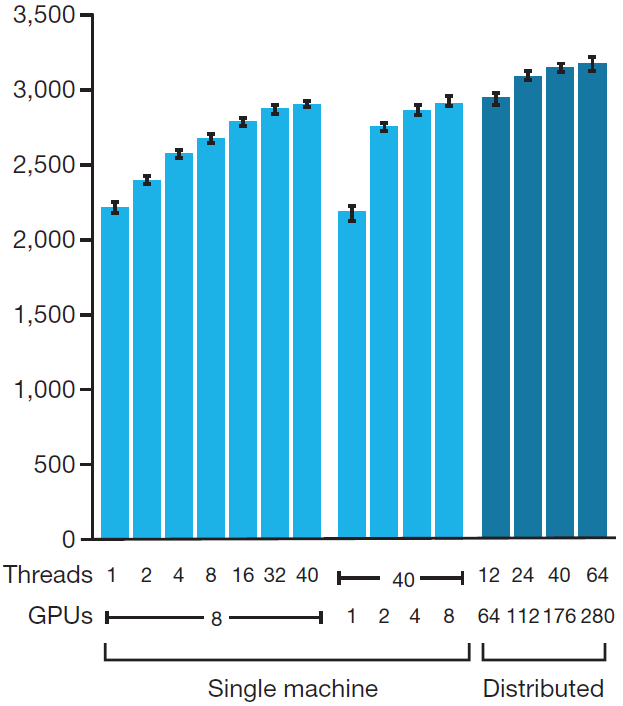
\includegraphics[height=.9\textheight]{../img/ELO_ratings_various_combinations_of_threads.png}
      \end{center}
    \end{frame}
  }

  % TODO display (I), (II) instead of i, ii
  \begin{frame}[allowframebreaks]{Further Reading}
    \tiny
    % TODO fill in relevant Further Reading
    % Machine Learning:
    % \begin{itemize}
    %   \item \textbf{Deep Learning} (\cite{Lecun2015deep})
    %   \item \textbf{Deep Learning course} \url{https://www.udacity.com/course/deep-learning--ud730}
    % \end{itemize}
  \end{frame}

  \begin{frame}[allowframebreaks]{References}
    \tiny
    \printbibliography[heading=none]
  \end{frame}

\end{document}
